\documentclass[12pt, oneside, openany]{book}

\usepackage{mathptmx} % Contiene una fuente similar a Times New Roman

\usepackage[spanish, es-tabla]{babel} % Permite escritura en castellano
\usepackage[utf8]{inputenc} % Permite utilizar caracteres UTF8

\usepackage{graphicx} % Para la inclusión de gráficos e imágenes
\graphicspath{ {images/} } % Ruta para buscar las imágenes
\usepackage[a4paper,top=30mm,left=30mm,right=25mm,bottom=25mm,headheight=20mm]{geometry} % Configuración de los margenes de la página

\PassOptionsToPackage{table}{xcolor}

% Paquetes para que funcione el formato.
\usepackage{xcolor}
\usepackage{plantuml}
\usepackage{tikz}
\usepackage[toc,page]{appendix}
\usepackage{titlesec}
\usepackage{multirow}
\usepackage{setspace}
\usepackage{ragged2e}
\usepackage{fancyhdr}
\usepackage{lastpage}
\usepackage{stackengine}
\usepackage{array}
\usepackage[hidelinks]{hyperref}
\usepackage{enumitem}
\usepackage{float}
\usepackage{hypcap}
\usepackage{caption}
\usepackage{fancyvrb}
\usepackage{textcomp}
\usepackage{listings}
% Se define un color gris desde su código RGB
\definecolor{gris}{RGB}{220,220,220}

\setcounter{secnumdepth}{3} % Para permitir numerar las sub-subsecciones

% Modifica el nombre de los índices al castellano
\addto\captionsspanish{
  \renewcommand{\contentsname}{Índice de contenido}
  \renewcommand{\listfigurename}{Índice de figuras}
  \renewcommand{\listtablename}{Índice de tablas}
  \renewcommand{\lstlistingname}{Listado}
  \renewcommand{\lstlistlistingname}{Índice de listados}
}

% Formateo de los nombres de los apartados:
\titleformat{\chapter}[block]
{\normalfont\Huge\bfseries\singlespacing}{\thechapter.}{1em}{\Huge}
\titlespacing*{\chapter}{0pt}{-62pt}{0pt}

\titleformat{\section}[block]
{\normalfont\Large\bfseries}{\thesection.}{4pt}{\Large}
\titlespacing*{\section}{0pt}{\baselineskip}{0pt}

\titleformat{\subsection}[block]
{\normalfont\large\bfseries}{\thesubsection.}{4pt}{\normalsize\large}
\titlespacing*{\subsection}{0pt}{0pt}{0pt}

\titleformat{\subsubsection}[block]
{\normalfont\normalsize\bfseries}{\thesubsubsection.}{4pt}{\normalsize}
\titlespacing*{\subsubsection}{0pt}{0pt}{0pt}

\def\tablename{Tabla}

%% Variables para portada y cabeceras
%% Cambiar los valores para cada documento!!!
\def\title{Explotación, integración y visualización de múltiples fuentes de datos mediante un Data Lake}
\def\shortTitle{ETL de datos heterogéneos mediante un Data Lake}
\def\subject{Lenguajes y Sistemas Informáticos}
\def\author{Mier Montoto, Juan Francisco}
\def\date{julio 2024}
\def\org{Escuela Politécnica de Ingeniería de Gijón}
\def\area{Grado en Ingeniería Informática en Tecnologías de la Información}
\def\tutorOne{D. Augusto Alonso, Cristian}
\def\tutorTwo{D. Morán Barbón, Jesús}
\def\tutorThree{D. Vázquez Faes, Eduardo}
\def\tfgId{???}

\def\ORG{\expandafter\MakeUppercase\expandafter{\org}}
\def\AREA{\expandafter\MakeUppercase\expandafter{\area}}
\def\SUBJECT{\expandafter\MakeUppercase\expandafter{\subject}}


\captionsetup{justification=centering}
\setlength{\headheight}{65pt}

\fancyhf{}
\fancyhead[L]{
\includegraphics[height=16mm]{style/square.png}
  \hspace{1em} \Longstack[l] {
    \textbf{\SUBJECT} \newline
    \textbf{\shortTitle}}
  \newline \leftmark{}
}
\fancyhead[R]{\bfseries{Hoja \hyperlink{toc}{\thepage}~de~\pageref{LastPage}}}
\fancyfoot[C]{\author}
\renewcommand{\headrulewidth}{0pt} % default is 0pt
\renewcommand{\footrulewidth}{0.4pt} % default is 0

\fancypagestyle{plain}{%
  \fancyhf{}
  \fancyhead[L]{
\includegraphics[height=16mm]{style/square.png}
    \hspace{1em} \Longstack[l]{
      \textbf{\SUBJECT} \newline
      \textbf{\shortTitle}}}
  \fancyhead[R]{\bfseries{Hoja \hyperlink{toc}{\thepage}~de~\pageref{LastPage}}}
  \fancyfoot[C]{\author}
  \renewcommand{\headrulewidth}{0pt} % default is 0pt
  \renewcommand{\footrulewidth}{0.4pt} % default is 0pt
}

\newcommand*{\fullref}[1]{\textit{\hyperref[{#1}]{\ref*{#1} \nameref*{#1}}}}

\pagestyle{fancy}

\restylefloat{table}
\definecolor{backcolour}{rgb}{0.95,0.95,0.92}
\definecolor{darkgreen}{rgb}{0.0, 0.5, 0.0}

\lstdefinestyle{default}{
  basicstyle=\ttfamily\footnotesize,
  breakatwhitespace=false,
  breaklines=true,
  captionpos=b,
  keepspaces=true,
  numbers=left,
  numbersep=5pt,
  numberstyle=\tiny\color{black},
  showspaces=false,
  showstringspaces=false,
  showtabs=false,
  tabsize=2,
  backgroundcolor=\color{backcolour},
  postbreak=\mbox{\textcolor{red}{$\hookrightarrow$}\space},
}

\lstset{style=default}

\lstdefinestyle{yaml}{
  basicstyle=\ttfamily\footnotesize\color{darkgreen}\bfseries,
  rulecolor=\color{black},
  string=[s]{'}{'},
  stringstyle=\color{darkgreen},
  comment=[l]{:},
  commentstyle=\color{blue},
  morecomment=[l]{-},
  numbers=left,
  numbersep=5pt,
  numberstyle=\tiny\color{black},
  backgroundcolor=\color{backcolour},
  breaklines=true,
  captionpos=b,
  keepspaces=true,
  showspaces=false,
  showstringspaces=false,
  showtabs=false,
  tabsize=2,
  breakatwhitespace=true,
  postbreak=\mbox{\textcolor{red}{$\hookrightarrow$}\space},
}



\begin{document}

\rmfamily % Fuente tipo Romana
\begin{titlepage}
    \centering
    \bfseries {
        \null{}
        \vspace{0cm}
        \begin{table}[h]
            \centering
            \begin{tabular}{m{10cm} m{1cm} m{3cm}}
                \vspace{0.2cm}
                
\includegraphics[width=86mm]{style/full.png} &  & \vspace{1.52mm} 
\includegraphics[width=23mm]{style/square.png} \\
            \end{tabular}
        \end{table}

        \vspace{3\baselineskip}

        \Large{\ORG{} \\ \vspace{3\baselineskip}}
        \large {
            \AREA{} \\ \vspace{3\baselineskip}
            \subject{} \\ \vspace{2\baselineskip}

            TRABAJO FIN DE GRADO/MÁSTER Nº \tfgId{} \vspace{\baselineskip} \\
            \title{} \\ \vspace{1\baselineskip}

            \author{} \\ \vspace{1\baselineskip}
            TUTORES:\\
            \tutorOne{} \\
            \tutorTwo{} \\
            \tutorThree{} \\ \vspace{\baselineskip}

            \vspace{2\baselineskip}
            FECHA:\@ \date{}
        }
    }
\end{titlepage}
 % Portada de la memoria

% Índice de contenido
\addcontentsline{toc}{chapter}{Índice de contenido} % Añade la referencia al índice de contenido
\hypertarget{toc}{}
\tableofcontents
\newpage{}

% Índice de figuras
\newpage{}
\addcontentsline{toc}{chapter}{Índice de figuras}  % Añade la referencia al índice de contenido
\hypertarget{lof}{}
\listoffigures

% Índice de tablas
\newpage{}
\addcontentsline{toc}{chapter}{Índice de tablas}  % Añade la referencia al índice de contenido
\hypertarget{lot}{}
\listoftables
\newpage{}

\justify{} % Texto justificado
\setlength{\parskip}{\baselineskip} % Separación entre párrafos de 1 linea
\onehalfspacing{}

%% El contenido de la memoria, dividido en capítulos:
\chapter{Introducción}\label{chap:intro}
El proyecto que se presenta en este documento tiene como objetivo la
automatización de despliegue de la infraestructura y procesos que permitan hacer
un análisis masivo de datos. Para conseguir este objetivo, se analizan las
necesidades de la empresa y sus antecedentes, se valoran las tecnologías y
herramientas disponibles y se plantea una solución que permita la integración,
almacenamiento y análisis de grandes volúmenes de datos, provenientes de
múltiples fuentes y en diferentes formatos.

\section{Antecedentes}\label{sec:antecedentes}
Hoy en día, nos encontramos en una era donde la generación y almacenamiento de
datos crece exponencialmente \footnote{
	\url{https://www.statista.com/statistics/871513/worldwide-data-created/}
}, un hecho que se ve reflejado en el ámbito empresarial. La diversidad de
fuentes y formatos de estos datos introduce una complejidad significativa en su
manejo, conocida como \textit{heterogeneidad} \footnote{
	\url{https://www.sciencedirect.com/topics/computer-science/data-heterogeneity}
}, siendo las bases de datos, archivos de registros y APIs las fuentes más
habituales.

El término \textit{big data} describe este fenómeno de acumulación masiva de
datos, cuya magnitud y complejidad sobrepasan las capacidades de los métodos de
procesamiento convencionales. El \textit{big data} se caracteriza por tres
características principales: volumen, variedad y velocidad - su adecuada gestión
y análisis pueden otorgar ventajas competitivas significativas a las empresas,
tales como el descubrimiento de patrones ocultos, identificación de nuevas
oportunidades de mercado y optimización de procesos de toma de decisiones.

Uno de los procesos que permite la extracción de esta información es la pirámide
DIKW, \cite{enwiki:1211227190} es un modelo que describe la relación entre los
datos, la información, el conocimiento y la sabiduría. Según este modelo, los
datos son la materia prima de la información, que a su vez es la materia prima
del conocimiento, que a su vez es la materia prima de la sabiduría. Una
organización sin los procesos adecuados para la gestión y análisis de estos
datos, se enfrenta a importantes desafíos, como la dificultad para identificar
patrones y tendencias, la toma de decisiones incorrectas y la pérdida de
oportunidades de negocio. Por otro lado, una organización que logre extraer
información valiosa de sus datos, podrá mejorar su eficiencia, aumentar su
competitividad y adaptarse mejor a un entorno empresarial en constante cambio.

La evolución tecnológica ha propiciado el desarrollo de innovadoras herramientas
y metodologías diseñadas para enfrentar estos desafíos. Entre ellas, los
\textit{data lakes} (o \emph{lagos de información}) se destacan por su capacidad
para consolidar vastos volúmenes de datos heterogéneos, facilitando su posterior
análisis y aprovechamiento de manera más efectiva.

Sin embargo, a pesar de que existen herramientas de almacenamiento, el proceso
de integración, visualización y análisis de estos datos es una tarea desafiante,
ya que requiere de una gran cantidad de recursos y de un tiempo de desarrollo
considerable del que, normalmente, no se dispone en el ámbito empresarial.

Con la ingesta masiva de datos, se presentan nuevos problemas a la hora de
analizar y obtener información de ellos:

\begin{itemize}
	\item \textbf{Decisiones de negocio erróneas debidas a un mal tratamiento:}
		sin la necesaria automatización y correcta aplicación de los procesos
		ETL~(ver \ref{sec:etl}), al tratarse de un crecimiento exponencial de los datos y, por lo
		tanto, de la fuerza de trabajo necesaria para manejarla, los resultados
		del análisis pueden ser incorrectos, lo que deriva en errores y
		decisiones de negocio equivocadas que impactan negativamente en la
		empresa.
	\item \textbf{Heterogeneidad de los datos:}
		la heterogeneidad de los datos, tanto en formato como en origen,
		dificulta su consolidación y análisis, ya que requiere de un proceso de
		integración y transformación previo para homogeneizarlos y poder
		analizarlos de forma conjunta.
	\item \textbf{Grandes cantidades de información:}
		la masificación de información impide el análisis manual de los
		mismos, requiriendo resúmenes estadísticos o representaciones gráficas
		como \textit{dashboards} para su correcta interpretación.
		La visualización de datos es una técnica que permite representar la
		información de manera visual, para facilitar su análisis y comprensión,
		una parte vital del proceso de análisis de datos, ya que permite
		identificar patrones, tendencias y anomalías en los mismos de forma más
		rápida y sencilla.
\end{itemize}

\newpage{}
\section{Motivación}\label{sec:motivacion}
Okticket, como el resto de empresas, se enfrenta a la necesidad de unificar, gestionar y
analizar grandes volúmenes de datos, provenientes de múltiples fuentes y en
diferentes formatos. La correcta gestión y análisis de estos datos es
fundamental para la toma de decisiones y para la mejora de los procesos internos
de la empresa.

En la actualidad, la empresa dispone de una gran cantidad de datos que se
encuentran en diferentes formatos y en diferentes ubicaciones, lo que dificulta
su análisis y explotación. Por otra parte, se depende de la consulta manual o de
servicios de terceros para poder analizar estos datos, lo que supone un coste
adicional.

El proyecto surge de la necesidad de la empresa de extraer información y
conocimiento de las múltiples y heterogéneas fuentes de datos de las que se
disponen, tanto internas (e.g.~bases de datos, archivos de registros, APIs,
entre otros), como externas (e.g. APIs o datos de webs de terceros, datos de
fuentes públicas\ldots).

Además del uso interno, la empresa también quiere ofrecer a sus clientes la
posibilidad de consultar estos datos de forma visual y sencilla, para que puedan
analizarlos y explotarlos de forma autónoma, lo que supondría un valor añadido
para los mismos.

\newpage{}
\section{La empresa}\label{sec:empresa}
Okticket es una startup nacida en Gijón en 2017 cuyo producto principal es un
servicio software que escanea automáticamente tickets y facilita su gestión usando conceptos
contables como notas de gastos, anticipos y más. Esto
permite reducir los costes y el tiempo que invierten las empresas en
contabilizar y manejar los gastos de viaje profesionales.

La empresa tienen su suede principal en el Parque Tecnológico de Gijón, aunque
cuenta con un número de sedes creciente en varios países, como Francia, Portugal
o, más recientemente, México. En esta oficina principal se encuentran los
departamentos de ventas y marketing, así como el equipo de desarrollo y consultoría.

Okticket es una de las empresas que más crecen tanto del sector como del propio
Parque Tecnológico. Debido a este rápido crecimiento, el equipo está en
constante desarrollo y cambio, tanto aquí en España como en el resto de sedes.
Este crecimiento se refleja en la recepción de un gran número de galardones y
reconocimientos.
\footnote{\href
	{https://www.linkedin.com/posts/okticket_okticket-en-el-especial-startups-de-forbes-activity-7140622980618903552-UGWK}
	{Okticket en el especial startups 2023 de Forbes (LinkedIn)}
}
\footnote{\href
	{https://www.elcomercio.es/economia/arcelor-okticket-premios-20230222002438-ntvo.html}
	{Arcelor y Okticket, premios nacional de Ingeniería Informática (EL COMERCIO)}
}
\footnote{\href{
	https://www.okticket.es/blog/empresa-pyme-innovadora}
	{Okticket recibe el sello Pyme Innovadora (okticket.es)}
}
\footnote{\href
	{https://www.okticket.es/blog/okticket-empresa-emergente-certificada}
	{Okticket, empresa emergente certificada (okticket.es)}
}

La parte principal del negocio es el núcleo del software como servicio (Software
as a Service en inglés, en adelante \textit{SaaS}), es decir, la aplicación
completa tanto para administradores como para empleados. Este SaaS se oferta a
empresas de cualquier tamaño, cuyo precio final varía en función del número de
usuarios, las características e integraciones que requiera la empresa cliente y
el soporte que se ofrezca.

Recientemente se han añadido nuevas propuestas a la cartera de servicios
ofertada por Okticket, como la OKTCard {-} una tarjeta inteligente que gestiona
automáticamente los gastos, así como la inclusión de nuevos ``módulos'' de
gestión de gastos y viajes.

Debido al crecimiento acelerado de Okticket, la empresa maneja una gran cantidad
de datos de diversos tipos y almacenados en diferentes silos (programas de
gestión contable, ventas, consultoría, así como los datos que genera el SaaS),
que deben ser unificados para poder ser analizados y explotados de forma eficiente.
Por otra parte, actualmente se depende de la consulta manual o de servicios de
terceros para poder analizar estos datos, lo que es costoso, tedioso y muy
poco eficiente.

\section{Objetivos}\label{sec:objetivos}
El objetivo del proyecto es la creación de un proceso que permita el despliegue
automático de una infraestructura de datos que permita la integración,
almacenamiento y análisis de grandes volúmenes de datos, provenientes de
múltiples fuentes y en diferentes formatos. La infraestructura de datos debe ser
escalable, flexible y robusta, para poder adaptarse a las necesidades cambiantes
de la empresa.

La infraestructura de datos debe permitir la integración de datos de múltiples
fuentes, tanto internas como externas, y en diferentes formatos, como bases de
datos, archivos de registros, APIs, entre otros. La integración de datos debe
ser automática y programable, para poder automatizar el proceso de ingestión de
datos y reducir el tiempo y los costes asociados.

Pese a que el entregable principal de este proyecto es la creación de una
infraestructura, se esperan también otros entregables en forma de herramientas
de software, como \textit{scripts}, que faciliten la integración y análisis de
los datos, así como la visualización de los mismos.

\chapter{Fundamento teórico}\label{chap:teo}
En este capítulo se presentan los conceptos y términos fundamentales que se utilizan en el
proyecto, para proporcionar una base teórica sobre la que se desarrolla el trabajo. Se discuten
los conceptos de \textit{data lake}, \textit{procesos ETL} y \textit{dashboards}, que son
fundamentales para el desarrollo del proyecto.

\section{\textit{Big data}}\label{sec:bigdata}
El término \textit{big data} se refiere a la gestión y análisis de grandes volúmenes de datos
que no pueden ser tratados de manera convencional. Estos datos se caracterizan por su volumen,
velocidad y variedad, lo que hace que sea difícil procesarlos con las herramientas tradicionales
de gestión de datos.

El \textit{big data} se caracteriza por tres características principales: volumen, variedad y
velocidad. Estas características se conocen como las ``tres V'' del \textit{big data}:

\begin{itemize}
	\item \textbf{Volumen:} se refiere a la cantidad de datos que se generan y almacenan en un
		determinado periodo de tiempo. El volumen de datos que se maneja en el \textit{big data}
		es mucho mayor que el que se maneja en los sistemas tradicionales de gestión de datos.
	\item \textbf{Variedad:} se refiere a la diversidad de fuentes y formatos de los datos que
		se manejan en el \textit{big data}. Los datos pueden provenir de diferentes fuentes, como
		bases de datos, archivos de registros y APIs, y pueden estar en diferentes formatos, como
		texto, imágenes, audio, vídeo, etc.
	\item \textbf{Velocidad:} se refiere a la velocidad a la que se generan y se procesan los
		datos. En este ámbito, los datos se generan y se procesan a una velocidad mucho
		mayor que en los sistemas tradicionales de gestión de datos.
\end{itemize}

El \textit{big data} es un fenómeno que ha surgido en los últimos años debido al crecimiento
exponencial de los datos que se generan y almacenan en todo el mundo. Este crecimiento ha
sido impulsado por el aumento de la conectividad y el uso de dispositivos móviles, que han
permitido a las empresas y a los usuarios generar y almacenar grandes cantidades de datos
de manera más eficiente.


\section{Paradigmas de almacenamiento de datos}\label{sec:paradigmas}
En el ámbito del \textit{big data}, existen diferentes paradigmas de almacenamiento de datos
que se utilizan para almacenar y analizar grandes cantidades de información. Los tres paradigmas
a considerar para este proyecto son los \textit{data warehouses}, los \textit{data lakes} y los
\textit{data lakehouses}.

\subsection{Data warehouse}\label{sec:warehouse}
Un \textit{data warehouse}\footnote{\url{https://aws.amazon.com/es/data-warehouse/}},
también conocido en español como almacén de datos, es una base de datos que se utiliza para
almacenar y analizar grandes cantidades de datos de manera eficiente. Los almacenes de datos
proporcionan acceso rápido y compatible con plataformas de consultas (como SQL) a grandes
cantidades de datos, lo que permite a los analistas y a los científicos de datos realizar
análisis complejos sobre los datos almacenados.

Todos los datos almacenados en un \textit{data warehouse} se encuentran en un formato común,
para lo que se aplican procesos ETL (extracción, transformación y carga) que transforman los
datos de diferentes fuentes en un formato común. Esto significa que la información se
encuentra en un formato o esquema optimizado y específico, lo que facilita su manipulación y
análisis pero limita la flexibilidad al acceso de los datos y genera costes adicionales en
el caso de tener que modificar o transferir los mismos para su uso.


\subsection{Data lake}\label{sec:lake}
Los \textit{data lakes}\footnote{\url{https://aws.amazon.com/es/what-is/data-lake/}}
son almacenes de datos que guardan grandes cantidades de datos de manera no
estructurada~\cite{mier2023dashboards}. En el ámbito de una empresa, un \textit{data lake}
contiene datos de diferentes fuentes de valor no considerado hasta su análisis, de manera
que su explotación posterior y su análisis no depende de una estructuración y transformación
compleja, reduciendo los costes de los procesos ETL derivados, una flujo de tareas que se
aplican sobre la información para ingestarla. Esto no quiere decir que no se apliquen estos
procesos a los datos, sino que se aplican de manera más flexible y básica que en otras
estructuras de almacenamiento de datos con esquemas predefinidos, como los
\textit{data warehouses}.~\cite{pwint2018data}

A diferencia de los \textit{data warehouses}, los \textit{data lakes} no tienen un
esquema definido, lo que permite almacenar datos \textit{heterogéneos}. Esto permite
almacenar grandes cantidades de información sin tener que definir un esquema de antemano,
lo que puede ser útil en aquellos casos en los que no se conoce la estructura de los
datos que se van a almacenar.

Estas características de los \textit{data lakes} hacen que sean más atractivos en el sector
empresarial de cara al análisis de información, en contraste con las estructuras planteadas
normalmente en el campo de la investigación académica.

Para consultar esta gran cantidad de datos almacenados, se suelen utilizar técnicas de
visualización de datos, como los \textit{dashboards}, herramientas de visualización que
permiten observar los datos de manera sencilla y eficiente.

\subsection{Data lakehouse}\label{sec:lakehouse}
Los \textit{data lakehouses} son una combinación funcional de los dos paradigmas vistos
anteriormente, los \textit{data lakes} y los \textit{data warehouses}. Los \textit{data
lakehouses} permiten almacenar datos tanto de manera estructurada como no estructurada,
lo que facilita aprovechar la información al contar con una única estructura de bajo coste
que ofrece a los usuarios que lo necesiten explorar y analizar los datos según sus necesidades.

% Puesto que en este proyecto se plantea el uso de datos tanto estructurados como no estructurados,
% y no siempre será de interés aplicar procesos de transformación a toda la información obtenida,
% los \textit{data lakehouse} se presentan como una solución eficiente y flexible para el almacenamiento
% y análisis de los datos.

\newpage{}
\section{Procesos ETL}\label{sec:etl}
Si anteriormente se presentaban los distintos paradigmas de almacenamiento de datos, para su creación
y mantenimiento se requieren aplicar unos ciertos procesos que permitan la correcta ingesta y
almacenamiento de los datos. Estos procesos se conocen como \textit{procesos ETL}.

Formalmente se definen los procesos ETL~\cite{mier2023dashboards} como procesos que combinan datos de
múltiples fuentes en un único destino, transformando los datos en un formato común. Estos procesos
se utilizan para extraer datos de diferentes fuentes, transformarlos en un formato común
y cargarlos en un destino común, como puede ser un \textit{data lake}.

% \subsection{Características}
Los procesos ETL, fundamentales en el ámbito de la gestión de datos, presentan atributos
distintivos que facilitan la integración eficaz de información procedente de diversas fuentes:

\begin{itemize}
	\item \textbf{Adaptabilidad:} los procesos ETL deben de adaptarse a la estructura de los
		datos de la fuente de origen, ya que dichas fuentes pueden tener diferentes estructuras
		y tener tipos de datos diferentes (la característica de \textit{heterogeneidad} de los
		datos que ya se ha mencionado).
	\item \textbf{Escalabilidad:} otra de las características clave de los procesos ETL es que sean
		escalables, ya que los datos que se muestran en los dashboards suelen ser datos que se generan
		de manera continua, y por lo tanto los procesos ETL deben ser capaces de procesar grandes
		cantidades de datos de manera eficiente. En ocasiones, los procesos ETL se pueden realizar en
		\textit{streaming}, lo que significa que los datos se procesan en tiempo real a medida que se
		generan.
	\item \textbf{Eficiencia:} los procesos ETL deben ser eficientes, puesto que el tiempo de procesamiento
		de los datos es un factor vital en el ámbito del \textit{big data}. Los procesos ETL deben ser
		capaces de procesar grandes cantidades de datos en un tiempo razonable para que los datos estén
		disponibles en el menor tiempo posible.
	\item \textbf{Fiabilidad:} la fiabilidad es un componente crítico de todo el flujo de datos, ya que estos
		se utilizan para la toma de decisiones importantes de cualquier empresa. Los procesos ETL deben
		ser capaces de procesar los datos de manera fiable y consistente, para que los datos que se visualicen y
		analicen posteriormente sean correctos y fiables.
\end{itemize}

\newpage{}
\subsection{Funcionamiento}
Los procesos ETL se dividen en tres fases principales: \textit{(1) Extraer}, \textit{(2) Transformar} y
\textit{(3) Cargar}, como se muestra en el siguiente diagrama:

\begin{minipage}{\linewidth}
	\centering
	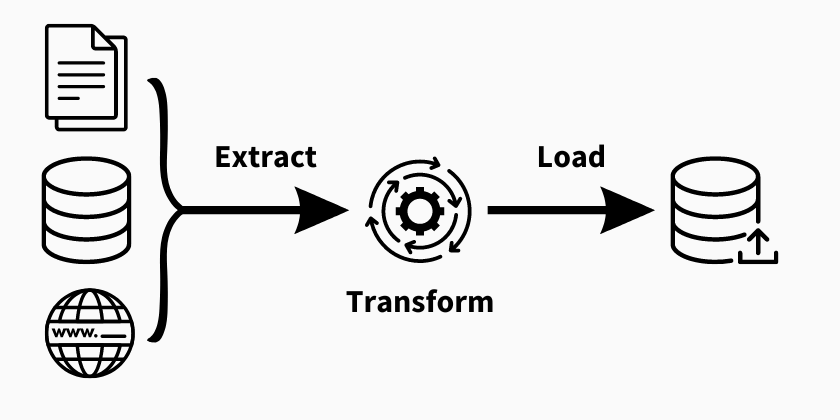
\includegraphics[width=0.8\textwidth]{etl.png}
	\captionof{figure}{Fases de un proceso ETL}
\end{minipage}

Como entrada, se tienen datos presúntamente heterogéneos que no se pueden analizar de manera eficiente.
Tras aplicar todos los pasos de las fases anteriores, se obtiene como salida un conjunto de
datos homogéneos y listos para ser analizados en el destino indicado (en el caso de este proyecto,
un \emph{data lake}).

\paragraph{Extracción (1)}
En este proceso se obtienen los datos de las fuentes de datos, que pueden ser bases de datos, logs,
APIs, etc. En esta fase, se pueden aplicar filtros para extraer solo los datos que se necesiten, y
se pueden extraer datos de múltiples fuentes \emph{heterogéneas}.

La fase de extracción se puede realizar de dos formas: continua o incremental. Una extracción incremental se
realiza de manera periódica, por ejemplo, cada hora, cada día o cada semana, y se extraen los datos
que se han generado desde la última extracción. Esto es útil cuando los datos se generan de manera
periódica y se necesita mantener actualizada la información. Por otro lado, en una extracción continua se
extraen los datos entiempo real según se van generando. Esto puede ser útil para procesar datos que se generan
en tiempo real, como logs o datos de sensores.

\newpage{}
\paragraph{Transformación (2)}
Durante esta fase, se transforman los datos extraídos en la fase anterior, normalmente aplicándoles
un proceso de limpieza y transformación a un formato común. En este paso, se pueden aplicar
diferentes operaciones a los datos, como la limpieza, la agregación, la normalización, la conversión
de formatos, etc.

Uno de los tipos de transformaciones de datos más comunes es la limpieza, que consiste en la
revisión y corrección de los datos extraídos, para asegurar que se almacena información correcta y
consistentes. Durante esta fase se contemplan operaciones más complejas, como pueden ser la agregación
de datos, la conversión de formatos, la normalización de datos, el cifrado, etc. La limpieza de datos puede
ser una tarea muy sencilla, como la eliminación de caracteres delimitadores, o muy compleja, como la
corrección de errores en los datos o la detección de duplicados.

Estos procesos de transformación son vitales cuando el sistema maneja una gran cantidad de datos heterogéneos
de múltiples fuentes de manera simultánea, como puede ser el caso de un \textit{data lake} o un \textit{data
warehouse}. En el caso del primero, no es necesaria la transformación de los datos a un formato común, pero si
otros procesos clave como la limpieza y la normalización de los datos, entre otros.

\paragraph{Carga (3)}
En este proceso se vuelcan los datos transformados en el destino final. Frecuentemente, los datos se
almacenan, dependiendo del paradigma de almacenamiento elegido, en una \textit{data lake}, \textit{data warehouse}
o \textit{data lakehouse} para su posterior análisis.

\newpage{}
\subsection{Alternativas}
Aunque lo más común es el flujo anteriormente explicado de \textit{extracción}, \textit{transformación} y
\textit{carga}, existen algunos flujos y procesos alternativos que evitan algunos de estos pasos, normalmente
en casos específicos que se beneficien del cambio:

\begin{itemize}
	\item \textbf{Virtualización de datos:} capa virtual de abstracción que permite acceder a los datos de las
		fuentes sin necesidad de extraerlos. Esto permite ahorrar espacio de almacenamiento y tiempo de procesamiento,
		pero suele ser menos eficiente en términos de rendimiento y no es compatible con todas las arquitecturas de
		datos.

		\begin{minipage}{\linewidth}
			\centering
			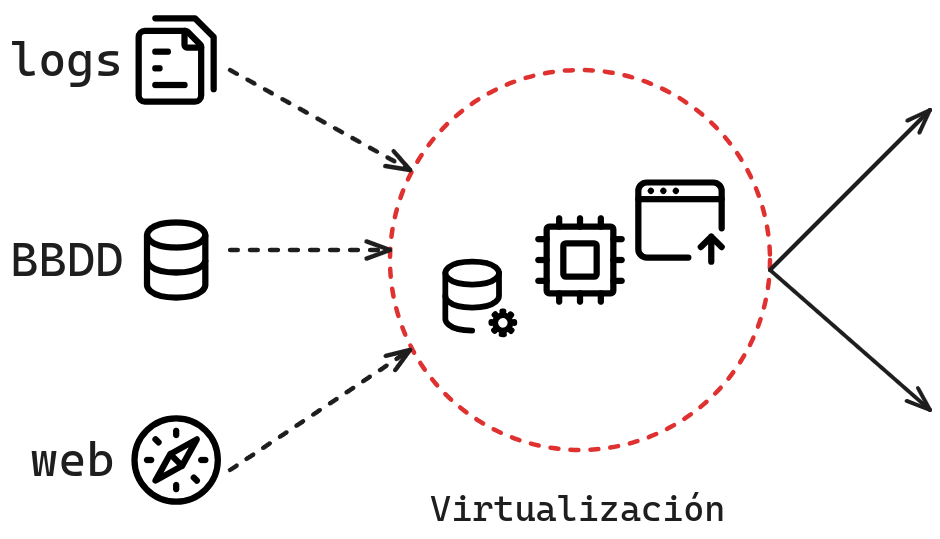
\includegraphics[width=0.65\textwidth]{virt.png}
			\captionof{figure}{Ejemplo de flujo con virtualización}
		\end{minipage}
	\item \textbf{Proceso \textit{ELT}\footnote{\url{https://www.ibm.com/topics/elt}}:} en lugar de transformar
		los datos antes de cargarlos en el destino, se cargan los datos en bruto y se transforman en el destino.
		Funciona bien para grandes conjuntos de datos sin estructura que requieran una carga (o recarga) contínua,
		aunque, al igual que la virtualización, puede ser menos eficiente o incompatible con algunas arquitecturas
		de datos, como los \textit{data warehouses}.

		\begin{minipage}{\linewidth}
			\centering
			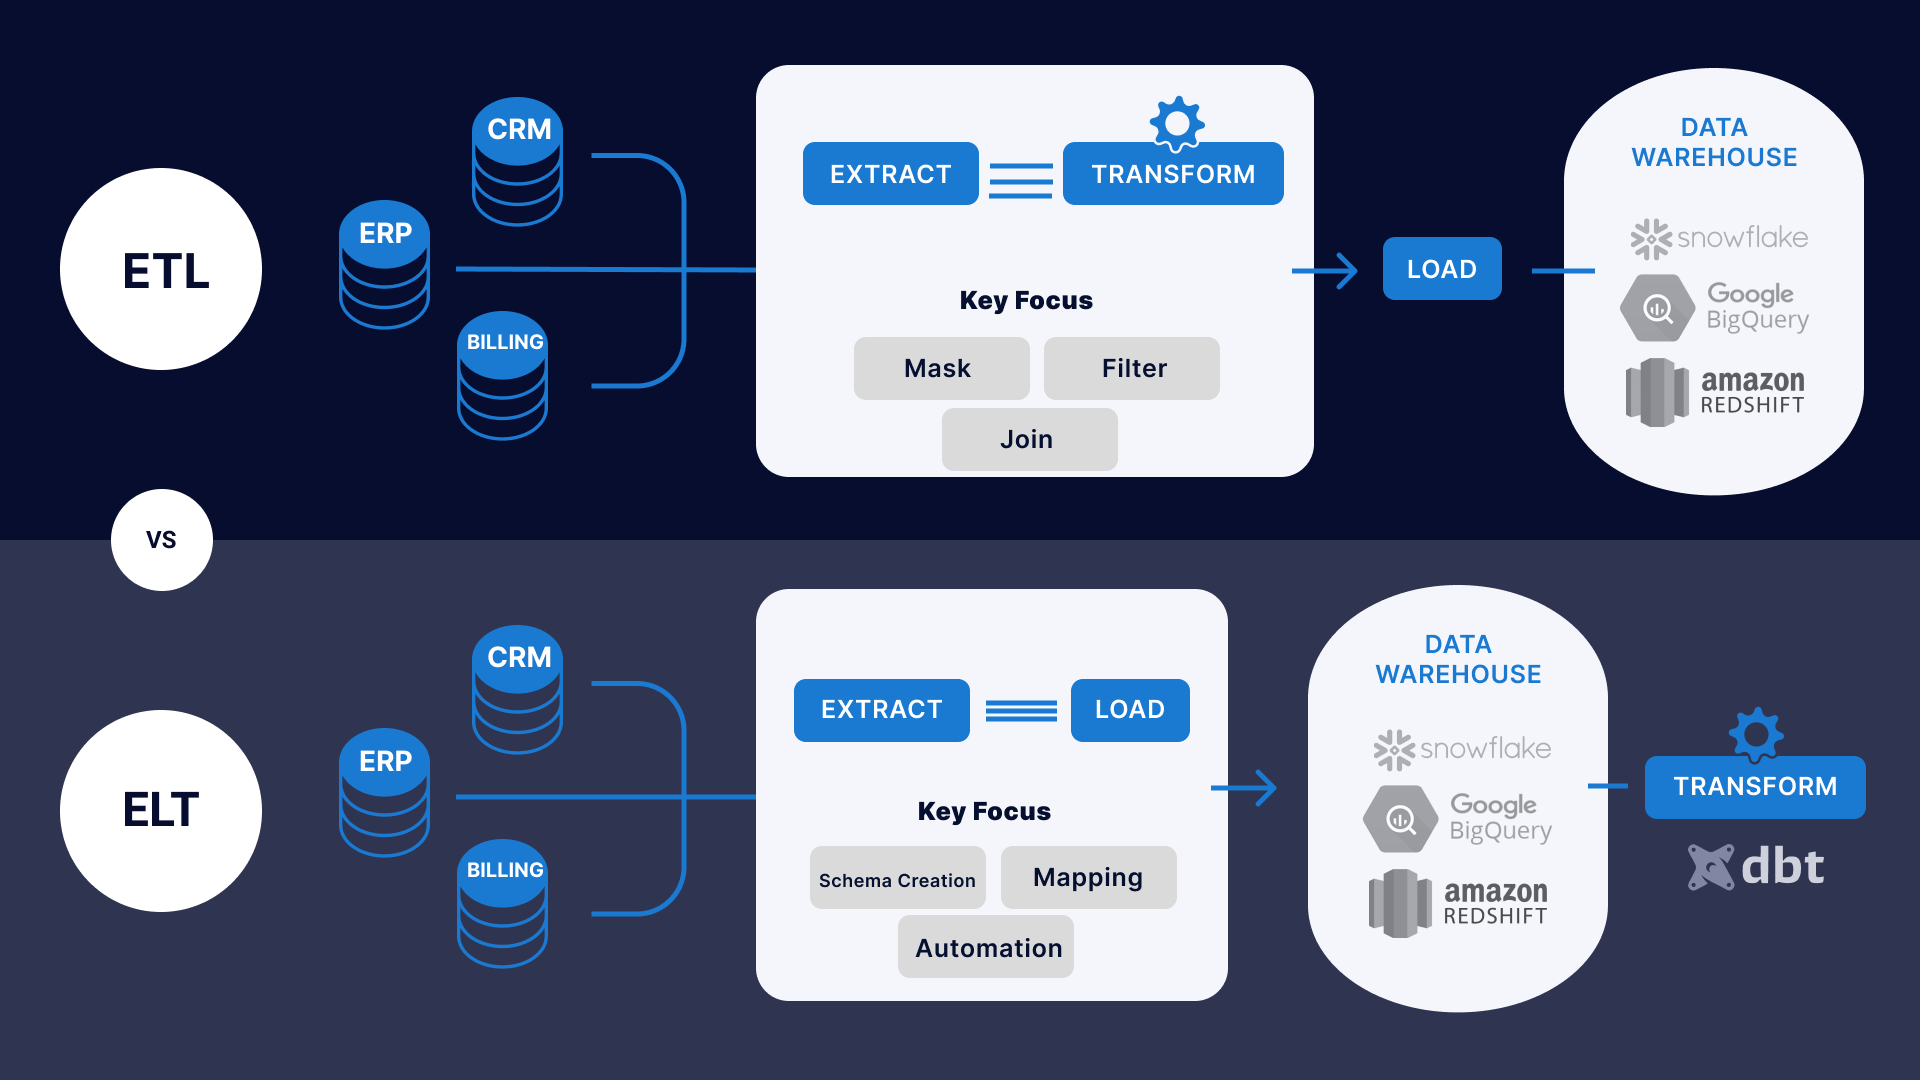
\includegraphics[width=0.75\textwidth]{elt.png}
			\captionof{figure}{Diagrama de flujo de un proceso \textit{ELT}}
		\end{minipage}
\end{itemize}


\newpage{}
\section{Cuadros de mandos (\textit{dashboards})}\label{sec:dashboards}
\paragraph{Definición}
Los cuadros de mandos, en adelante \textit{dashboards},
es un término que se utiliza para referirse a cualquier interfaz gráfica que muestre información
relevante de manera visual sobre un proceso o negocio. Aunque el término se utiliza en
muchos ámbitos: indicadores comerciales, de producción, de marketing, de calidad, de recursos
humanos\ldots, en este proyecto se utilizará en el ámbito de la monitorización de sistemas y
procesos de negocio.

En el ámbito de deste proyecto, los dashboards reflejan en tiempo real el rendimiento de
actividades o procesos de negocio, y se utilizan para tomar decisiones informadas basándose en
los mismos. Por ejemplo, el dashboard de una empresa digital puede mostrar desde el rendimiento de la
arquitectura en tiempo real hasta el número de ventas conseguidas, y permitir a los directivos tomar
decisiones informadas sobre el futuro de la empresa (e.g. necesidad de aumentar la capacidad de los
servidores, lanzar una campaña de marketing, etc.).

\paragraph{Características}
Los dashboards cuentan con una serie de características que los hacen útiles para la toma de
decisiones:~\cite{mier2023dashboards}

\begin{itemize}
	\item \textbf{Visualización de datos:} es la característica fundamental de cualquier
		dashboard, y aquella que determina su utilidad. La visualización de datos
		es la ciencia de presentar los datos de manera que se pueda extraer información útil
		y realizar decisiones informadas sobre ellos. Un buen dashboard cuenta con gráficas,
		tablas, indicadores, etc. que permiten al usuario entender la información que se
		está presentando con un conocimiento técnico mínimo.
	\item \textbf{Interactividad y personalización:} un dashboard debe permitir al usuario
		interactuar con los datos (filtrarlos, ordenarlos, profundizar en ellos...) y ajustar
		la información que se muestra sobre cada proceso o negocio que se esté evaluando
		(granularidad de la información). Esta capacidad asegura que el dashboard se adapte
		tanto a las necesidades actuales como a las evoluciones futuras de lo que se esté analizando.
	\item \textbf{Accesibilidad y portabilidad:} un dashboard debe ser accesible desde una
		variedad de situaciones y dispositivos, manteniendo su funcionalidad y forma. Aunque
		normalmente los dashboards se analizan en pantallas grandes, es importante que también
		se puedan consultar en otras circunstancias, como dispositivos móviles.
\end{itemize}

\newpage{}
\paragraph{Dashboards planteados}
Para el sistema que se describe, se plantean dos tipos de dashboards diferentes:

\begin{itemize}
	\item \textbf{Dashboards internos}: que reflejan el rendimiento de la plataforma en tiempo real.
		Estos dashboards están destinados al uso interno de la empresa, y permiten a los
		empleados monitorizar el rendimiento de la plataforma y tomar decisiones informadas
		sobre su mantenimiento y evolución.
	\item \textbf{Dashboards externos}: que reflejan el rendimiento de las ventas y permiten a los
	    clientes tomar decisiones informadas sobre su negocio. Estos dashboards están enfocados
		a los clientes de la empresa, y permite a los mismos obtener información relevante sobre
		su negocio que tenga Okticket.
\end{itemize}


\section{Infraestructura como código}
La infraestructura como código (o \textit{IaaS} por sus siglas en inglés) es una práctica que consiste
en gestionar la infraestructura de un sistema de manera automática y programática, utilizando código
en lugar de configuraciones manuales. La infraestructura como código permite gestionar la infraestructura
de manera eficiente y escalable, y facilita la creación y el mantenimiento de entornos de desarrollo y
producción.

En el ámbito de este proyecto, la infraestructura como código se utiliza para gestionar la infraestructura
de los sistemas de almacenamiento y procesamiento de datos, como los \textit{data lakes} y los \textit{data
warehouses}. La infraestructura como código permite gestionar la infraestructura de manera eficiente y
escalable, y facilita la creación y el mantenimiento de entornos de desarrollo y producción.


% mover esta sección a la valoración de alternativas cuando se tenga
% \section{Componentes del sistema}\label{sec:componentes}
% En el \textit{stack} tecnológico escogido para el proyecto se manejan
% diferentes términos y conceptos que son necesarios desarrollar para
% entender el funcionamiento del sistema.

% \subsection{Tópico}\label{subsec:topico}
% Un tópico es una categoría a la que se envían los mensajes a la que los consumidores están
% \textit{suscritos}. Los consumidores pueden estar suscritos a uno o varios tópicos, y los
% productores pueden enviar mensajes a uno o varios tópicos. Los tópicos son la unidad básica
% de organización de los mensajes en cualquier sistema de mensajería de publicación/suscripción.

% \subsection{Productor}\label{subsec:productor}
% El productor es el componente responsable de crear y enviar mensajes al cluster de Kafka.
% Está separado del resto de los componentes y produce mensajes de manera asíncrona y rápida.

% \subsection{Consumidor}\label{subsec:consumidor}
% El consumidor es el componente responsable de leer los mensajes producidos por el productor.
% Está suscrito a un \nameref{subsec:topico} a través del broker y consume los mensajes.

% \subsection{Broker}\label{subsec:broker}
% El broker es el componente responsable de recibir los mensajes producidos por el productor y
% enviarlos a los consumidores. Es el intermediario entre los productores y los consumidores.

% \subsection{Zookeeper}\label{subsec:zookeeper}
% Zookeeper es un servicio de coordinación distribuida que se utiliza para gestionar y coordinar
% los brokers de Kafka. Se encarga de mantener la información de los brokers y de los tópicos.

\chapter{Descripción general del proyecto}\label{chap:desc}
Esta sección describe el proyecto en términos generales, incluyendo una
descripción de los problemas que se pretenden resolver, las partes interesadas
en el proyecto y una valoración de las alternativas consideradas.


\section{Partes interesadas (\textit{stakeholders})}\label{sec:stakeholders}
Las partes interesadas en el proyecto son aquellas personas o entidades que
tienen un interés en el mismo, ya sea porque se ven afectadas por el resultado
del proyecto, o porque tienen algún tipo de interés en el mismo. Las partes
interesadas en este proyecto son las siguientes:

\begin{enumerate}
	\item \textbf{Okticket:} la empresa es la principal parte interesada en el
		proyecto, ya que es la que se beneficiará directamente de los resultados
		del mismo, así como de las oportunidades de negocio que se abren con la
		explotación de los datos. Dentro de la empresa, se pueden identificar
		varias entidades afectadas:
		\begin{itemize}
			\item \textbf{Equipo de desarrollo:} son los
				encargados de llevar a cabo la implementación del sistema y de
				garantizar su correcto funcionamiento, además de gestionar el
				soporte de servicio a nivel técnico.
			\item \textbf{Equipo de soporte:} el sistema planteado
				ahorraría tiempo al equipo de soporte, ya que les permitiría
				analizar los datos de forma más eficiente e identificar
				problemas antes de que tener que resolver las peticiones de los
				clientes afectados a nivel básico.
			\item \textbf{Equipo de negocio:} afectado porque permitirá tomar
				mejores decisiones estratégicas, definir y seguir métricas de
				seguimiento de los objetivos.
			\item \textbf{Éxito de clientes:} afectado porque le
				permitirá evaluar mejor a qué clientes dar seguimiento, mejorar
				el seguimiento, identificar oportunidades de \textit{upselling}
				\ldots
			\item \textbf{Equipo de operaciones:} afectado porque les permitirá
				hacer un mejor seguimiento de las operaciones y procesos de la
				empresa.
		\end{itemize}
	\item \textbf{Clientes}: se beneficiarán de los nuevos servicios que se
		ofrecen, como los dashboards de negocio que se han descrito
		anteriormente. Estos clientes no son necesariamente los usuarios
		finales, sino los administradores y gestores de las empresas que
		utilizan Okticket como herramienta de gestión de gastos.
	\item \textbf{Investigador y desarrollador (\emph{\author}):} el
		desarrollador del proyecto tiene la oportunidad de aplicar los
		conocimientos adquiridos en el desarrollo de un proyecto real, y de
		adquirir nuevos conocimientos en el proceso.
\end{enumerate}


\section{Alternativas existentes}\label{sec:alternativas}
Antes de comenzar la planificación y el desarrollo del proyecto, se consideran
varias opciones ya existentes en el mercado que podrían resolver o adaptarse a
las necesidades planteadas.


\subsection{Criterios de evaluación}
Los puntos claves a considerar de cada alternativa son los siguientes:

\begin{itemize}
	\item \textbf{Coste:} se dará prioridad a alternativas gratuitas, siempre
		que su coste de operación y mantenimiento no sea excesivo.
	\item \textbf{Complejidad:} se priorizarán aquellas alternativas que
		sean sencillas y no requieran una curva de aprendizaje excesiva para
		su implementación y uso.
	\item \textbf{Rendimiento y escalabilidad:} a la hora de manejar los
		volúmenes de datos con los que se están tratando, el sistema debe
		responder positivamente tanto a la ingesta, tratamiento y visualización
		como a la escalabilidad del mismo.
	\item \textbf{Licencias:} se priorizará el software de código abierto con el
		el objetivo de reducir el \textit{vendor lock-in} y permitir una mayor
		flexibilidad y personalización del sistema sin coste de uso.
\end{itemize}


\newpage{}
\subsection{Alternativas consideradas}
Para este proyecto, el análisis de alternativas se realiza en torno a las
herramientas y tecnologías disponibles en el mercado para la gestión de datos en
base a los criterios establecidos anteriormente. A continuación, se describen
las alternativas consideradas destacando puntos a favor, en contra y unas
breves conclusiones, además de una valoración final de las mismas.


\subsubsection{Elasticsearch, Logstash, Kibana (ELK)}
La pila ELK es una solución de código abierto que combina tres herramientas
diferentes: \textit{Elasticsearch}, \textit{Logstash} y \textit{Kibana}. Este
\textit{stack} tecnológico es ampliamente utilizado en la industria para la
gestión de logs y métricas, y ofrece una solución integral para la recopilación,
almacenamiento, búsqueda y visualización de datos.

\paragraph{Elasticsearch} es un motor de búsqueda y análisis de código abierto
que permite almacenar, buscar y analizar grandes volúmenes de datos de forma
rápida y eficiente.

\begin{figure}[H]
	\centering
	
\includegraphics[width=0.2\textwidth]{logos/elastic.png}
	\caption{Logo de Elasticsearch~\textregistered}
\end{figure}

\paragraph{Logstash} es una herramienta de procesamiento de logs que permite
recopilar, transformar y enviar logs de diferentes fuentes a Elasticsearch para
su análisis.

\begin{figure}[H]
	\centering
	
\includegraphics[width=0.2\textwidth]{logos/logstash.png}
	\caption{Logo de Logstash~\textregistered}
\end{figure}

\paragraph{Kibana} es una plataforma de visualización de datos que permite
crear dashboards interactivos y visualizaciones de datos a partir de los datos
almacenados en Elasticsearch.

\begin{figure}[H]
	\centering
	
\includegraphics[width=0.2\textwidth]{logos/kibana.png}
	\caption{Logo de Kibana~\textregistered}
\end{figure}

Juntas, estas herramientas forman una solución integral para la
gestión de logs y métricas, que permite a las empresas consolidar, monitorizar y
analizar datos de diferentes fuentes en tiempo real.

La principal ventaja de esta solución es su flexibilidad y capacidad de
personalización, que permite adaptarla a las necesidades específicas de cada
empresa. Además, al tratarse de herramientas de código abierto, la pila ELK es
una opción asequible y escalable que se adapta a las necesidades de la empresa.

En cuestión a la complejidad, la pila ELK puede resultar más compleja de
configurar y mantener en comparación con otras soluciones al requerir múltiples
componentes y una configuración detallada. Sin embargo, la comunidad activa y
los recursos disponibles pueden ayudar a superar estos desafíos.

Una desventaja de la pila ELK es su curva de aprendizaje, que puede ser
pronunciada para aquellos que no están familiarizados con las herramientas. Sin
embargo, una vez superada esta curva, la pila ELK ofrece una solución potente y
flexible para la gestión de información.


\newpage{}
\subsubsection{Graylog + Prometheus}
Esta combinación de herramientas es una alternativa interesante para la gestión
de datos en entornos de producción. Graylog es una plataforma de
gestión de logs de código abierto que permite centralizar, monitorizar y
analizar logs de diferentes fuentes. Por otro lado, Prometheus es un sistema de
monitorización y alertas de código abierto que se centra en la recopilación de
métricas de sistemas y aplicaciones.

\begin{figure}[H]
	\centering
	
\includegraphics[width=0.2\textwidth]{logos/graylog.png}
	\caption{Logo de Graylog~\textregistered}
\end{figure}

En este documento se tratan de manera combinada porque, aunque son herramientas
independientes, su integración es una solución completa que se está volviendo
popular en el sector. Graylog se encarga de la gestión de logs, mientras que
Prometheus se encarga de la recopilación de métricas y alertas.

La combinación de Graylog y Prometheus ofrece varios beneficios, como la
centralización de información que facilita un análisis más integral y
eficiente de los datos. Además, la mejora en la monitorización a través de las
capacidades avanzadas de Prometheus, integradas con Graylog, mejora la detección
de problemas y la respuesta a incidentes en tiempo real. Esta integración
también proporciona flexibilidad y escalabilidad, adaptándose a las necesidades
específicas de cada entorno de producción. Sin embargo, existen desventajas como
la complejidad de configuración al integrar dos sistemas independientes, lo que
puede resultar en un mayor esfuerzo en mantenimiento y gestión. Además, al
tratarse de herramientas novedosas, supondría una mayor curva de aprendizaje
para el equipo de desarrollo a la hora de tratar con las herramientas.


\newpage{}
\subsubsection{Loki}
Loki es una herramienta de gestión de logs desarrollada por Grafana Labs,
diseñada específicamente para ser altamente eficiente y escalable. A diferencia
de otras soluciones de gestión de datos, Loki no indexa el contenido completo de
estos, sino que se centra en los metadatos, lo que reduce significativamente
los requisitos de almacenamiento y mejora el rendimiento.

Al estar creado por Grafana Labs, Loki se integra de forma nativa con Grafana,
lo que facilita la visualización y análisis de los datos de logs en tiempo real.
Además, está inspirado en Prometheus y pensado para utilizar con
\textit{Kubernetes}.

\begin{figure}[H]
	\centering
	
\includegraphics[width=0.2\textwidth]{logos/loki.png}
	\caption{Logo de Loki~\textregistered}
\end{figure}

\paragraph{Ventajas}
\begin{itemize}
    \item \textbf{Integración con Grafana:} Una de las principales ventajas de
		Loki es su integración nativa con Grafana, una popular plataforma de
		visualización de datos. Esto permite a los usuarios crear paneles de
		control y alertas basados en los datos de logs de manera sencilla y
		eficiente.
    \item \textbf{Eficiencia en el almacenamiento:} Al no indexar el contenido
		completo de los logs, Loki reduce significativamente los requisitos de
		almacenamiento. Esto lo hace una opción más económica y eficiente en
		comparación con otras soluciones.
    \item \textbf{Escalabilidad:} Loki está diseñado para ser altamente
		escalable, lo que permite manejar grandes volúmenes de datos de logs sin
		comprometer el rendimiento.
    \item \textbf{Simplicidad en la configuración:} La configuración de Loki es
		relativamente sencilla, especialmente para aquellos que ya están
		familiarizados con Grafana y Prometheus. Esto facilita su adopción y
		despliegue en entornos de producción.
\end{itemize}

\paragraph{Desventajas}
\begin{itemize}
    \item \textbf{Limitaciones en la búsqueda:} Al no indexar el contenido
		completo de los logs, las capacidades de búsqueda de Loki son más
		limitadas en comparación con otras herramientas como Elasticsearch.
		Esto puede ser una desventaja en caso de necesitar realizar búsquedas
		complejas y detalladas.
    \item \textbf{Ecosistema en desarrollo:} Aunque Loki ha ganado popularidad
		rápidamente, su ecosistema y comunidad de usuarios aún están en
		desarrollo. Esto puede limitar el acceso a recursos y soporte en
		comparación con soluciones más maduras.
    \item \textbf{Dependencia de Grafana:} Si bien la integración con Grafana es
		una ventaja, es un factor limitante para aquellos que no utilicen
		Grafana, como es el caso de Okticket, al tener que adaptarse a un
		ecosistema diferente.
\end{itemize}

En resumen, Loki es una solución eficiente y escalable para la gestión de datos,
especialmente adecuada para aquellos que ya utilizan Grafana. Sin embargo, sus
limitaciones en la búsqueda y su ecosistema en desarrollo son factores a
considerar antes de su implementación.

\begin{figure}[H]
	\centering
	
\includegraphics[width=0.2\textwidth]{logos/prometheus.png}
	\caption{Logo de Prometheus~\textregistered}
\end{figure}


\newpage
\subsubsection{Loggly, Splunk (SaaS de gestión de logs)}
Ambas herramientas se centran en la gestión y análisis de logs basada en la nube,
permitiendo centralizar, monitorizar y analizar datos de logs en tiempo real.
Diseñadas para simplificar la gestión de logs, las dos alternativas ofrecen una
interfaz intuitiva y potentes capacidades de búsqueda y visualización que
facilitan la identificación y resolución de problemas en los sistemas y
aplicaciones.

\begin{figure}[H]
	\centering
	
\includegraphics[width=0.2\textwidth]{logos/loggly.png}
	\caption{Logo de Loggly~\textregistered}
\end{figure}

Una de las principales ventajas de este tipo de herramientas es su capacidad
para integrarse con una amplia variedad de servicios y plataformas, lo que
permite a las empresas consolidar sus datos de logs en un único lugar. Además,
suelen ofrecer algún sistema de alertas en tiempo real y paneles de control
personalizables, lo que encaja muy bien con algunos de los requisitos de este
proyecto.

Sin embargo, también presentan algunas desventajas que entran en conflicto con
los intereses descritos anteriormente. En primer lugar, al tratarse de
servicios enfocados en el tratamiento exclusivo de logs, podrían no acomodar
algunos de los requisitos esenciales, como la ingesta de las bases de datos
propias de la empresa.

\begin{figure}[H]
	\centering
	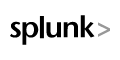
\includegraphics[width=0.2\textwidth]{logos/splunk.png}
	\caption{Logo de Splunk~\textregistered}
\end{figure}

Otra posible limitación es su sistema de precios; estas herramientas cuentan con
una jerarquía de suscripciones que limita mucho su escalabilidad y aumentaría
rápidamente los costes de su uso en caso de llegar a depender de ellas.

\newpage{}
En resumen, aunque tanto Loggly como Splunk o cualquier otro SaaS similar
sean soluciones robustas y eficientes para la gestión de logs, sus posibles
costes adicionales, junto con sus limitaciones en el análisis de datos de
inteligencia de negocio, las convierten en opciones menos atractivas para el
desarollo de este proyecto.


\subsection{Conclusiones}
Tras evaluar las alternativas consideradas, se concluye que ninguna de las
alternativas comerciales se ajusta completamente a los requisitos y necesidades
del proyecto. Si bien todas ellas ofrecen capacidades de gestión de logs y
métricas, ninguna de ellas proporciona una solución integral que cumpla con los
requisitos de integración, visualización y análisis de datos de negocio de
Okticket.

Por lo tanto, se considera que la mejor opción es desarrollar una solución
personalizada que se adapte a las necesidades específicas de la empresa. Esta
solución permitirá a Okticket consolidar y analizar datos de múltiples fuentes,
así como crear dashboards de negocio personalizados que faciliten la toma de
decisiones y la identificación de oportunidades de negocio.

Desde un principio, la empresa considera que el desarrollo junto a un
\textit{stack ELK} es la mejor opción para el desarrollo de este proyecto.
Aunque se considera que la integración de Prometheus y Grafana es una
alternativa interesante, se opta por la solución de \textit{stack ELK} debido a
su mayor flexibilidad y capacidad de personalización.

Además de la pila de \textit{Elastic}, se analizará más adelante la posibilidad
de integrar otras herramientas y tecnologías que puedan mejorar la eficiencia y
escalabilidad del sistema, como Kafka, Spark o Flink, entre otras.


\newpage{}
\section{Descripción del proyecto}\label{sec:descripcion}
\subsection{Dashboards planteados}
Para el sistema que se describe, se plantean dos tipos de dashboards diferentes:

\begin{itemize}
	\item \textbf{Dashboards internos:} que reflejan el rendimiento de la
		plataforma en tiempo real. Estos dashboards están destinados al uso
		interno de la empresa, y permiten a los empleados monitorizar el
		rendimiento de la plataforma y tomar decisiones informadas sobre su
		mantenimiento y evolución.
	\item \textbf{Dashboards externos:} que reflejan el rendimiento de las
		ventas y permiten a los clientes tomar decisiones informadas sobre su
		negocio. Estos dashboards están enfocados a los clientes de la empresa,
		y permite a los mismos obtener información relevante sobre su negocio
		que tenga Okticket.
\end{itemize}

\chapter{Planificación del proyecto}\label{chap:planif}
La planificación de un proyecto es fundamental para su correcto funcionamiento y
desarrollo, dentro de los plazos y costes establecidos. Se presenta un primer
apartado de metodología, un segundo apartado con la planificación inicial para
posteriormente inferir en base a esta el presupuesto.


\section{Metodología}\label{sec:metodología}
En este capítulo se aborda la metodología adoptada para el desarrollo del
proyecto, fundamentada en principios ágiles y enfocada en la entrega continua de
valor. La elección de \textit{Scrum}, una metodología que permite elaborar
productos software de manera incremental, revisando el producto continuamente y
adaptándolo a las necesidades del cliente, subraya el compromiso con la
adaptabilidad y la mejora continua del producto.

La estructura de este capítulo se organiza en torno a la descripción detallada
de la metodología \textit{Scrum}, la visualización de la planificación y las
estrategias de comunicación adoptadas. A través de esta metodología, se busca
optimizar los recursos disponibles, ajustarse a los plazos establecidos y
garantizar la calidad del producto final.

La implementación de \textit{Scrum} se complementa con herramientas de
visualización y gestión de proyectos, como los tableros \textit{Kanban}, que
facilitan la organización y seguimiento de las tareas. Además, se pone especial
énfasis en la comunicación efectiva dentro del equipo de desarrollo y con los
stakeholders, asegurando así una alineación constante con los objetivos del
proyecto.

Existen otras variantes de los tableros \textit{Kanban} que se pueden
utilizar para visualizar el progreso de las tareas, pero en este proyecto se ha
elegido esta alternativa para facilitar la visualización de las tareas y su
estado~(ver \fullref{subsec:visual_planif}). La visualización de la
planificación es esencial para el seguimiento y control del proyecto, ya que
permite identificar posibles desviaciones y tomar medidas correctivas de manera
temprana.

Este enfoque metodológico no solo refleja la planificación y ejecución del
proyecto, sino que también establece las bases para una gestión eficaz,
adaptativa y orientada a resultados.


\newpage{}
\subsection{Scrum}\label{subsec:scrum}
Para la planificación del proyecto se ha escogido \textit{Scrum}, una
metodología ``ágil'' que se basa en la realización de iteraciones cortas y en la
adaptación a los cambios. La metodología \textit{Scrum} se estructura en
\textit{sprints} (iteraciones cortas de una duración fija), en las que se llevan
a cabo una serie de tareas que se han planificado previamente.

El primer paso de la metodología \textit{Scrum} es la creación de un
\textit{product backlog}, una lista ordenada de las tareas a realizar durante el
desarrollo del producto, a partir de los requisitos del sistema, que a su vez
son una versión refinada de los requisitos iniciales del proyecto. A partir de
este \textit{product backlog} se planifican las tareas que se llevarán a cabo en
cada \textit{sprint}, de manera que sea posible cumplir con los objetivos del
proyecto en el tiempo establecido.

A diferencia de metodologías tradicionales o \emph{en cascada}, \textit{Scrum}
permite la adaptación a los cambios y la mejora continua del producto, ya que se
revisa y se adapta en cada \textit{sprint} según las necesidades del cliente y
del equipo de desarrollo. Por otro lado, \textit{Scrum} se diferencia de otras
metodologías ágiles como \textit{XP} en que no se centra tanto en las prácticas
de desarrollo, sino en la gestión del proyecto y en la entrega de valor al
cliente.

\begin{minipage}{\linewidth}
	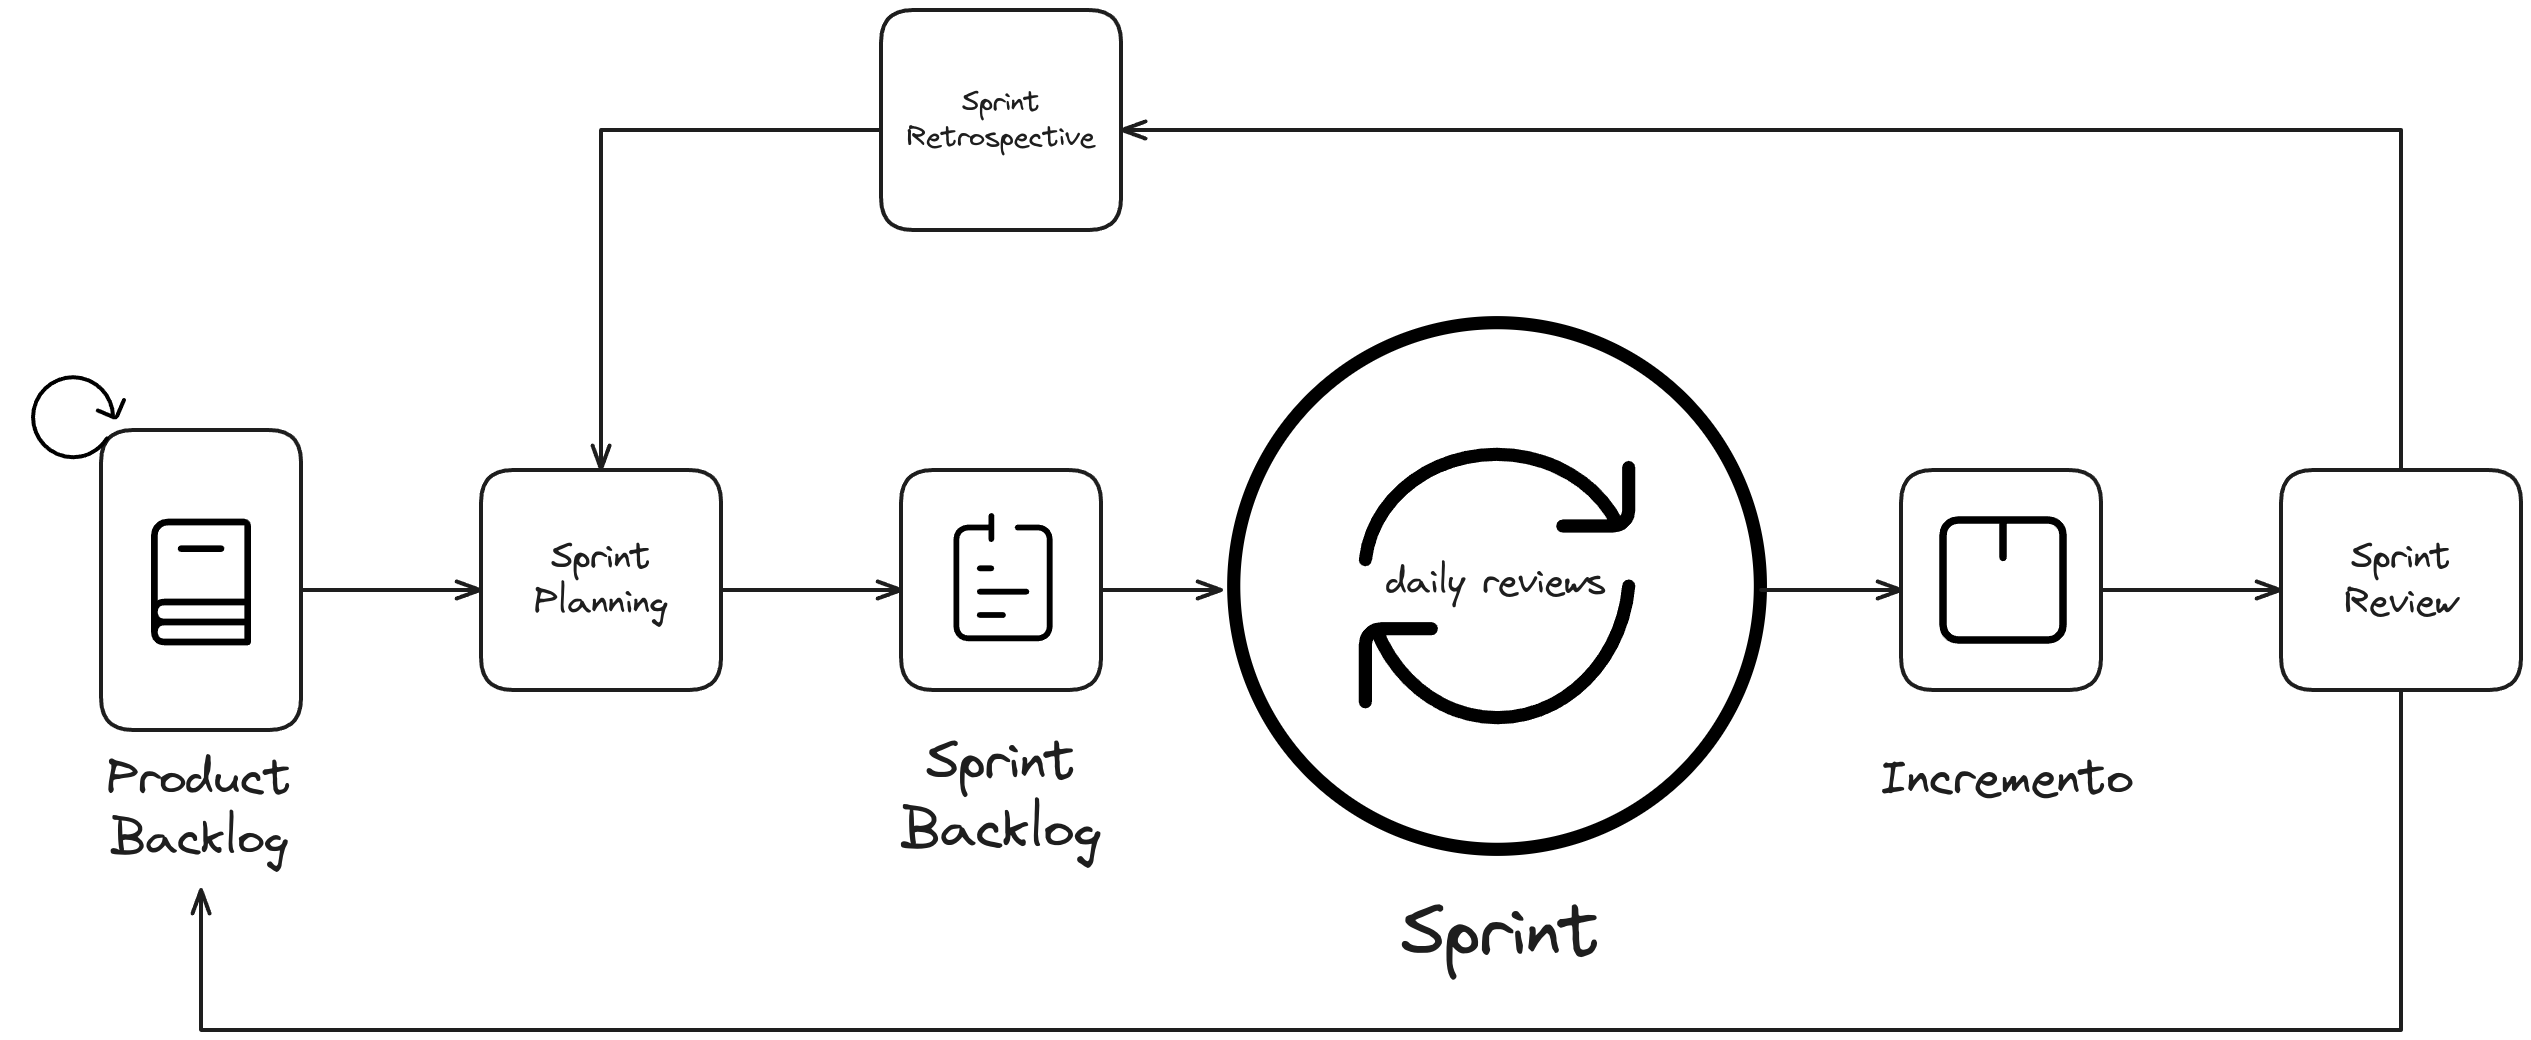
\includegraphics[width=0.85\textwidth]{scrum.png}
	\captionof{figure}{Diagrama de la metodología \textit{Scrum}}
\end{minipage}

\paragraph{Roles}
En \textit{Scrum} se distinguen tres roles principales:

\begin{itemize}
	\item \textbf{Product Owner:} es la persona responsable de definir los
		requisitos del producto y de priorizar las tareas del
		\textit{product backlog}. Es el enlace entre el equipo de desarrollo y
		el cliente, y es el responsable de garantizar que el producto cumple con
		las expectativas del cliente. En el caso de este proyecto, el
		\textit{Product Owner} es el director tecnológico de la empresa.
	\item \textbf{Scrum Master:} es la persona responsable de garantizar que el
		equipo de desarrollo sigue la metodología \textit{Scrum} y de eliminar
		los obstáculos que puedan surgir durante el desarrollo del proyecto. El
		\textit{Scrum Master} es el encargado de organizar las reuniones diarias
		y de asegurar que el equipo de desarrollo cumple con los plazos y los
		objetivos del proyecto. En este proyecto, el \textit{Scrum Master} son
		los tutores académicos del proyecto.
	\item \textbf{Equipo de desarrollo:} es el equipo encargado de llevar a cabo
		las tareas del \textit{product backlog} y de entregar el producto final.
		El equipo de desarrollo es autoorganizado y multidisciplinario, y se
		organiza en torno a las tareas que se van a realizar en cada
		\textit{sprint}. Para este proyecto, el ``equipo'' de desarrollo está
		constituido únicamente por el alumno, que se encarga de todas las tareas
		de desarrollo y documentación.
	\item \textbf{Stakeholders:} son las partes interesadas en el proyecto, como
		los clientes, los usuarios finales y los patrocinadores, que desconocen
		el proceso de desarrollo pero tienen un interés en el producto final y
		en su correcto funcionamiento.
\end{itemize}

\paragraph{Estimación}
En la metodología \textit{Scrum} se pueden utilizar diferentes técnicas de
estimación de tareas, como la estimación en puntos de historia, la estimación en
horas o la estimación en tallas de camiseta. En este proyecto se ha optado por
la estimación en tallas de camiseta, que consiste en asignar a cada tarea una
talla que representa su complejidad y su duración. Las tallas de camiseta se
suelen representar con letras (XS, S, M, L, XL), que se pueden traducir a puntos
de historia siguiendo la secuencia de Fibonacci, es decir, $XS = 1$, $S = 2$,
$M = 3$, $L = 5$, $XL = 8$.

La estimación en Scrum es esencial para la planificación de los \textit{sprints}
y para la asignación de tareas al equipo de desarrollo. La estimación en tallas
se considera óptima para este proyecto, ya que permite una estimación rápida y
sencilla de las tareas, al no necesitar una coordinación entre un equipo
completo de desarrollo.

Además de la estimación del tamaño de las tareas, también se realiza una
estimación sobre la \textit{prioridad} de las mismas, que se representa
siguiendo el equivalente de \textit{GitHub} al sistema de colores de semáforo,
donde el rojo (P0) es la máxima prioridad y el verde (P2) la mínima.

\newpage{}
\subsection{Visualización}\label{subsec:visual_planif}
Para la visualización de la planificación se ha utilizado la herramienta de
gestión de proyecto de \textit{GitHub}, que permite múltiples visualizaciones de
tareas e \textit{issues} en tableros separados.

\begin{itemize}
	\item Se utiliza un tablero de \textit{requisitos} al estilo \textit{Kanban}
		para visualizar los requisitos del proyecto y su estado, siguiendo con
		la metodología \textit{Scrum}. Un tablero \textit{Kanban} es una
		herramienta visual que permite gestionar el flujo de trabajo de un
		proyecto por ``sprints'', dividiendo las tareas en columnas y
		moviéndolas de una columna a otra según su estado.

		\begin{figure}[H]
			\centering
			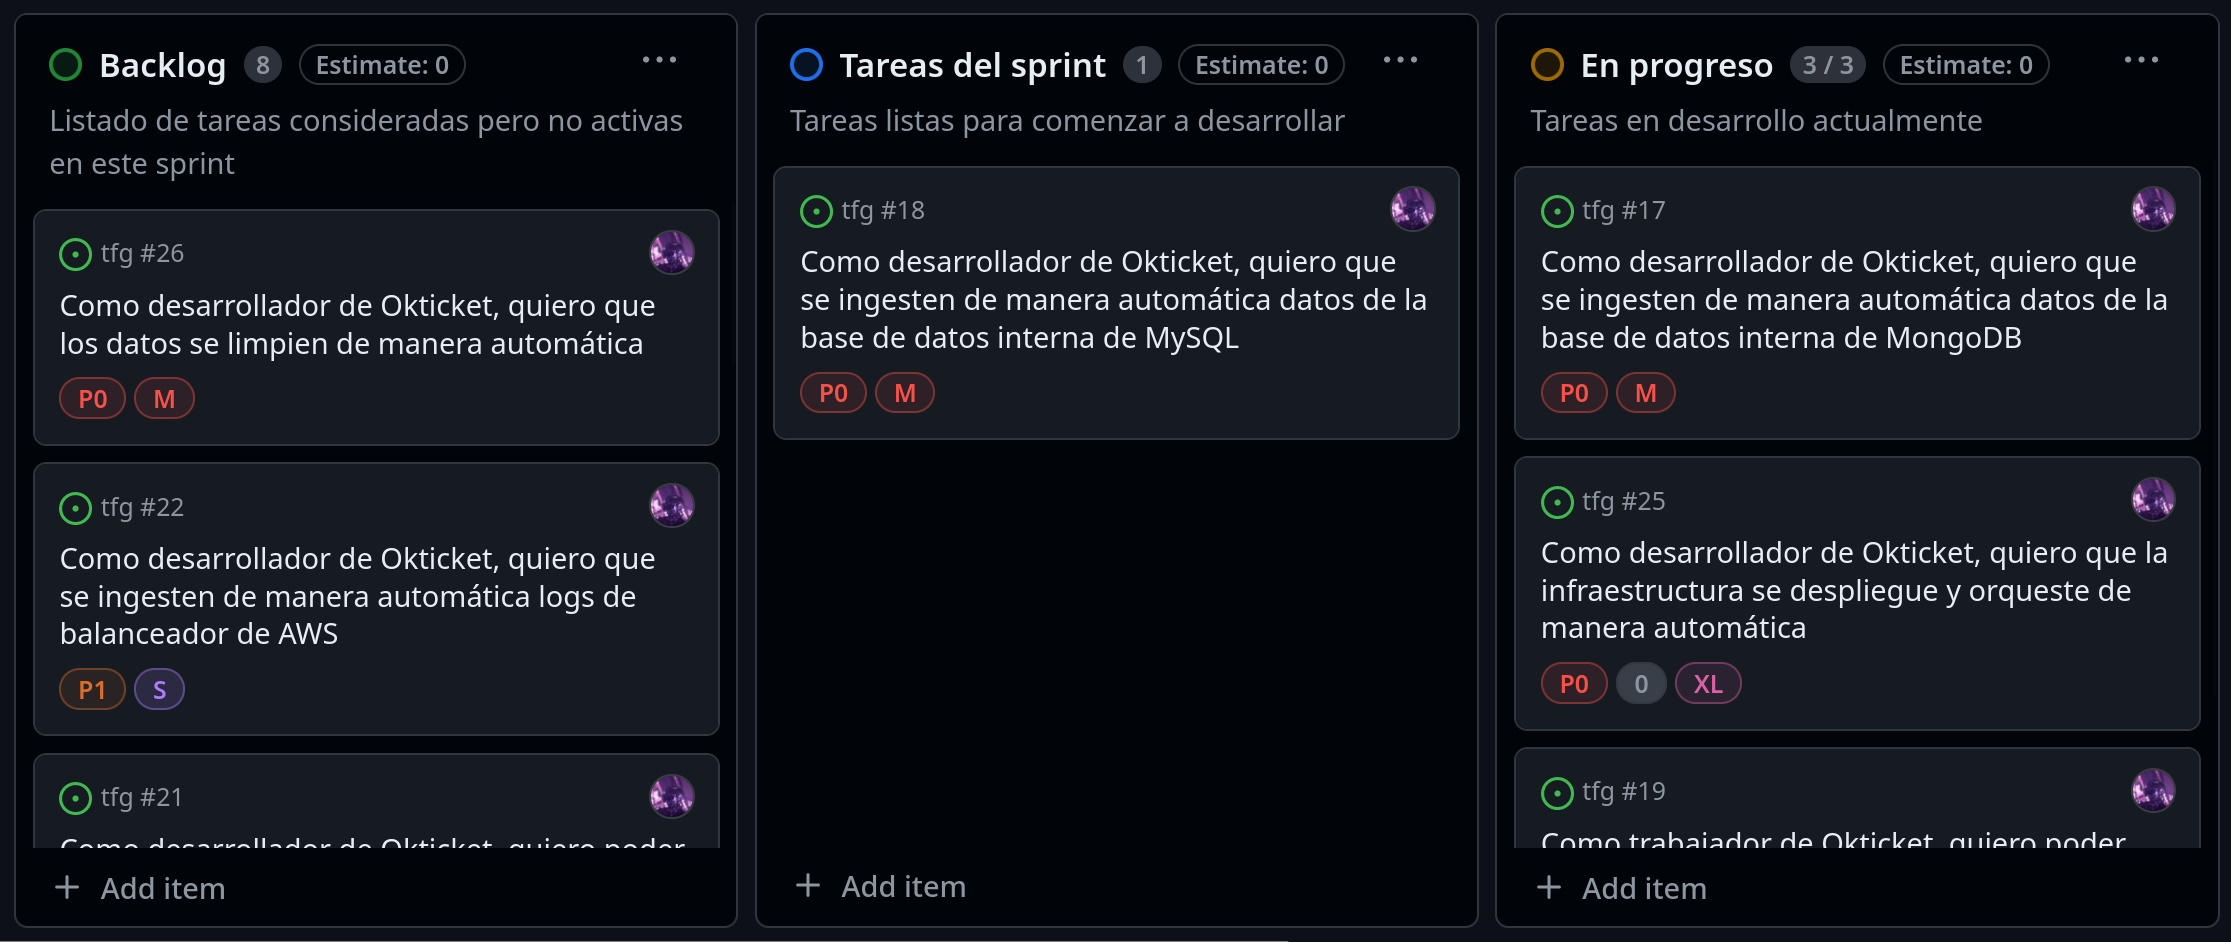
\includegraphics[width=\textwidth]{kanban3.png}
			\caption{Tablero \textit{Kanban} del proyecto}
			\label{fig:kanban}
		\end{figure}
	\item Adicionalmente, se utiliza un \textit{roadmap} de apartados de la
		memoria, separado del tablero de desarrollo normal, donde se visualiza
		su estado y sus fechas límite. Este \textit{roadmap} no está relacionado
		con la metodología \textit{Scrum}, sino que se ha creado para facilitar
		la visualización del progreso de cada sección y de la memoria en general.

		\begin{minipage}{\linewidth}
			\centering
			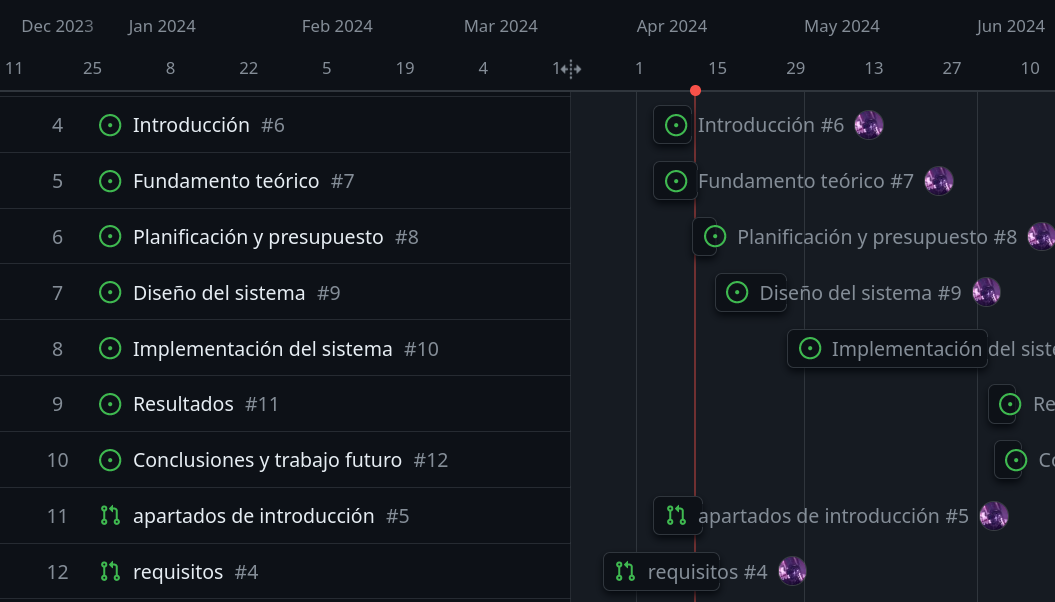
\includegraphics[width=0.9\textwidth]{roadmap.png}
			\captionof{figure}{Roadmap de apartados de la memoria}
		\end{minipage}
\end{itemize}


\subsection{Comunicación}\label{subsec:comunicación}
La comunicación con los tutores y con el equipo de desarrollo se considera
fundamental para el correcto desarrollo del proyecto. Puesto que el trabajo se
desarrolla de manera presencial en la oficina de la empresa, la comunicación con
el equipo de desarrollo se realiza de manera frecuente y directa, mientras que
la comunicación con los tutores se realiza de manera remota pero igual de
frecuente, manteniendo el contacto mediante correo electrónico y Teams para
pedir revisiones e informar sobre el estado del trabajo en todo momento.


\subsection{Herramientas}\label{subsec:herr_planif}
Con el objetivo de facilitar las tareas de desarrollo y cumplimentar los
requisitos por parte de la empresa, se utilizan las siguientes plataformas y
herramientas de desarrollo para la fabricación del proyecto:

\begin{itemize}
	\item \textbf{GitHub:} Plataforma de desarrollo colaborativo para el
		desarrollo del proyecto. Se utiliza para la gestión de tareas,
		seguimiento de desarrollo, documentación y colaboración.
	\item \textbf{Atlassian suite (\emph{Jira, Bitbucket}):} Suite de
		herramientas de gestión de proyectos y desarrollo colaborativo. Se
		utiliza para el desarrollo y documentación del proyecto de parte de la
		empresa.
	\item \textbf{Microsoft Teams:} Herramienta de comunicación y colaboración
		en tiempo real.
	\item \textbf{Microsoft Outlook:} Herramienta de comunicación por correo
		electrónico.
\end{itemize}


\newpage{}
\section{Planificación inicial}\label{sec:planif_inicial}
Como se ha mencionado anteriormente, se utiliza la metodología \textit{Scrum}
para la planificación y desarrollo del proyecto. En la figura \ref{fig:backlog}
se puede ver el \textit{backlog} de tareas que se planifican en el proyecto.

\begin{figure}[H]
	\centering
	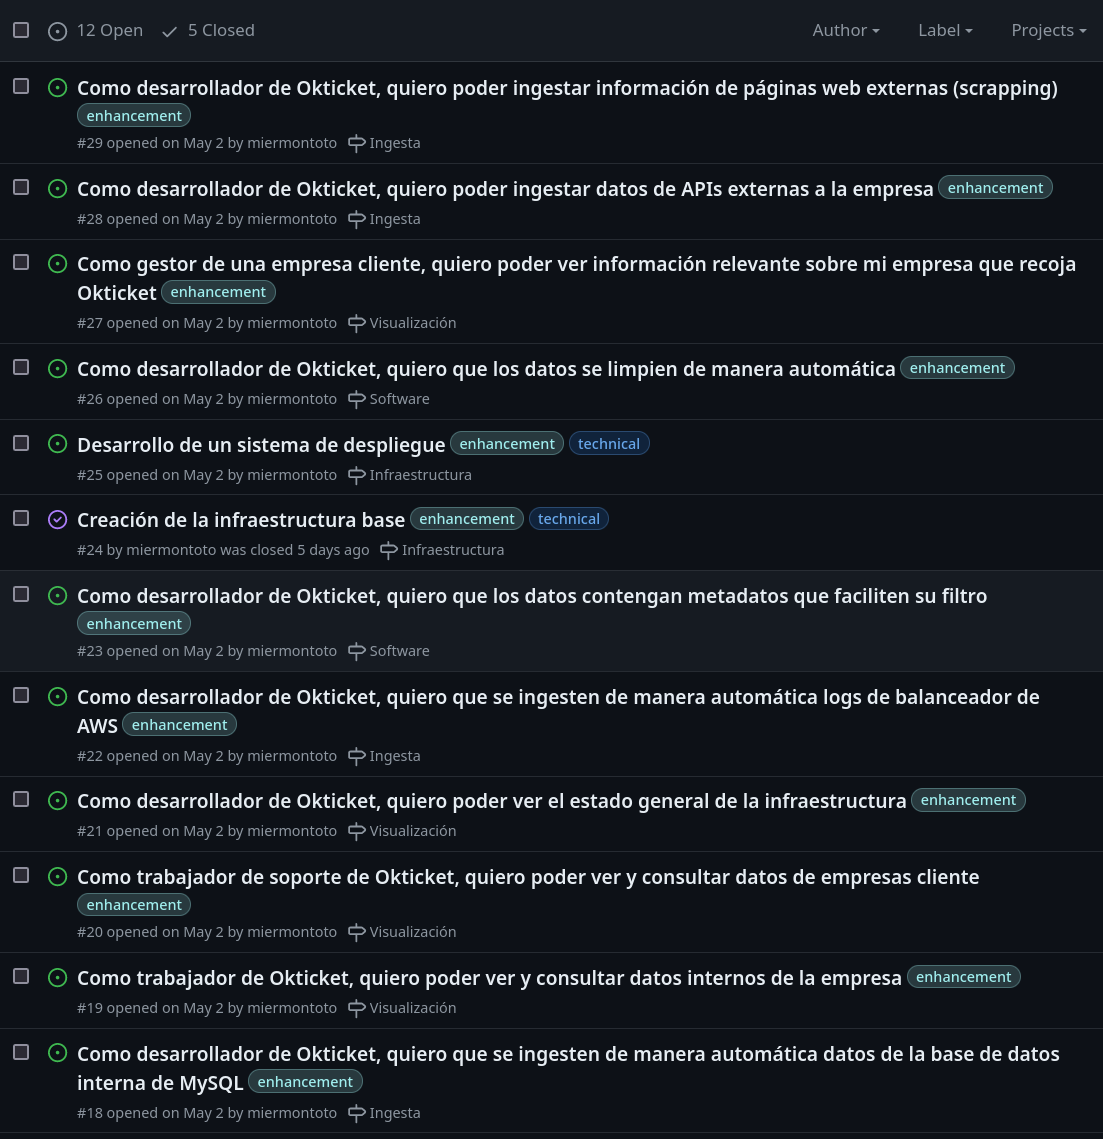
\includegraphics[width=\textwidth]{backlog.png}
	\caption{Planificación inicial del proyecto}
	\label{fig:backlog}
\end{figure}

Las tareas anteriores se clasifican y categorizan según su prioridad y tamaño,
haciendo uso de la estrategia de tallas de camiseta como mencionado
anteriormente. En el tablero \textit{Kanban} (ver figura \ref{fig:kanban}) se
puede ver en todo momento el estado de las tareas, su progreso y sus
características. El listado de tareas iniciales (ordenado según su prioridad)
es el siguiente:

\begin{table}[H]
	\centering
	\begin{tabular}{|p{0.7\linewidth}|c|c|}
		\hline
		\textbf{Tarea} & \textbf{Prioridad} & \textbf{Tamaño} \\
		\hline
		\hline
		Creación de la infraestructura base (técnica) & P0\cellcolor{red!50} & L\cellcolor{orange!50} \\
		\hline
		Como desarrollador de Okticket, quiero que la arquitectura se despliegue y orqueste de manera automática & P0\cellcolor{red!50} & XL\cellcolor{red!50} \\
		\hline
		Como desarrollador de Okticket, quiero que se ingesten de manera automática datos de la base de datos interna de MongoDB & P0\cellcolor{red!50} & M\cellcolor{yellow!50} \\
		\hline
		Como desarrollador de Okticket, quiero que se ingesten de manera automática datos de la base de datos interna de MySQL & P0\cellcolor{red!50} & M\cellcolor{yellow!50} \\
		\hline
		Como desarrollador de Okticket, quiero que los datos se limpien de manera automática & P0\cellcolor{red!50} & M\cellcolor{yellow!50} \\
		\hline
		Como trabajador de Okticket, quiero poder ver y consultar datos internos de la empresa & P1\cellcolor{orange!50} & L\cellcolor{orange!50} \\
		\hline
		Como desarrollador de Okticket, quiero que se ingesten de manera automática logs de balanceador de AWS & P1\cellcolor{orange!50} & S\cellcolor{green!25} \\
		\hline
		Como desarrollador de Okticket, quiero poder ver el estado general de la infraestructura & P1\cellcolor{orange!50} & L\cellcolor{orange!50} \\
		\hline
		Como desarrollador de Okticket, quiero que los datos contengan metadatos que faciliten su filtrado o búsqueda & P2\cellcolor{yellow!50} & S\cellcolor{green!25} \\
		\hline
		Como trabajador de Okticket, quiero poder ver y consultar datos de empresas cliente & P2\cellcolor{yellow!50} & M\cellcolor{yellow!50} \\
		\hline
		Como gestor de una empresa cliente, quiero poder ver información relevante sobre mi empresa que recoja Okticket & P2\cellcolor{yellow!50} & L\cellcolor{orange!50} \\
		\hline
		Como desarrollador de Okticket, quiero poder ingestar datos de APIs externas a la empresa & P2\cellcolor{yellow!50} & L\cellcolor{orange!50} \\
		\hline
		Como desarrollador de Okticket, quiero poder ingestar información de páginas web externas (\textit{scraping}) & P2\cellcolor{yellow!50} & XL\cellcolor{red!50} \\
		\hline
	\end{tabular}
	\caption{Listado de tareas iniciales}
	\label{tab:initial_tasks}
\end{table}

Siguiendo la tabla anterior, se pueden planear los \textit{sprints} y
asignar las tareas a cada uno de ellos.


\newpage{}
\section{Presupuesto}\label{sec:presupuesto}
Para poder llevar a cabo este proyecto, se realiza una estimación del coste
total neceario para su desarrollo, que se divide en dos partes: el coste del
material, que incluye el coste de los recursos necesarios para el desarrollo del
proyecto, y el coste del personal, que incluye el coste de las horas de trabajo
del desarrollador.


\subsection{Presupuesto de material}\label{subsec:pres_material}
Puesto que el proyecto se desarrolla en la empresa, se dispone de todos los
recursos físicos necesarios para llevar a cabo el proyecto, es decir, que no se
incluirá el coste del ordenador o de la conexión a internet en el presupuesto.

Sin embargo, se incluirá el coste de las herramientas y servicios utilizados
durante el desarrollo del proyecto, como el coste de las licencias de software,
el coste de los servicios en la nube, el coste de las herramientas de
desarrollo, etc.

Es importante destacar de que los precios de los servicios en la nube son
aproximados y pueden variar en función de la región, el tipo de instancia, el
tipo de almacenamiento, etc. Por lo tanto, los precios presentados en este
presupuesto son orientativos y pueden variar en función de las necesidades del
proyecto. En este caso, se analizan los precios en junio de 2024 en la región
de Amazon Web Services (AWS) de \textit{eu-west-3} (París).

\begin{table}[H]
	\centering
	\small
	\begin{tabular}{|l|l|r|r|r|}
	\hline
	\textbf{Categoría} & \textbf{Ítem} & \textbf{Cantidad} & \textbf{Coste unitario} & \textbf{Coste total} \\
	\hline
	\hline
	AWS Compute & Fargate & 500 vCPU-h/mes & 0,04665€/vCPU-h & 23,33€ \\
	 & & 1000 GB-h/mes & 0,00511€/GB-h & 5,11€ \\
	\hline
	AWS Storage & EFS & 500 GB/mes & 0,36€/GB-mes & 180,00€ \\
	 & S3 & 250 GB/mes & 0,0245€/GB-mes & 6,13€ \\
	\hline
	AWS Network & VPC & 4 NAT Gateways & 0,052€/h & 149,76€ \\
	 & ELB & 4 ALBs & 0,0243€/h & 70,00€ \\
	\hline
	AWS Security & IAM & - & Sin cargo & 0,00€ \\
	 & KMS & 1 CMK & 1,00€/mes & 1,00€ \\
	\hline
	Stack KELK & Kafka & - & Licencia gratuita & 0,00€ \\
	 & Elasticsearch & - & Licencia gratuita & 0,00€ \\
	 & Logstash & - & Licencia gratuita & 0,00€ \\
	 & Kibana & - & Licencia gratuita & 0,00€ \\
	\hline
	AWS Container & ECS & - & Sin cargo & 0,00€ \\
	\hline
	AWS Monitor & CloudWatch & 5 métricas & 0,30€/métrica-mes & 1,50€ \\
	 & X-Ray & 50,000 trazas/mes & 4,60€/1M trazas & 0,23€ \\
	\hline
	Despliegue & Terraform & - & Licencia gratuita & 0,00€ \\
	\hline
	Capacitación & Cursillo online & 1 & 184,00€ & 184,00€ \\
	\hline
	\textbf{Subtotal} & \multicolumn{4}{r|}{620,06€} \\
	\hline
	\hline
	Otros & Support & Plan Basic & Sin cargo & 0,00€ \\
	 & Optimización & - & 5\% del subtotal & 31,00€ \\
	 & Contingencia & - & 10\% del subtotal & 62,00€ \\
	\hline
	\textbf{Total} & \multicolumn{4}{r|}{713,06€} \\
	\hline
	\end{tabular}
	\caption{Propuesta de presupuesto de materiales}
	\label{tab:presupuesto_material}
\end{table}


\newpage{}
\subsection{Presupuesto de personal}\label{subsec:pres_personal}
A continuación, se presenta una propuesta de presupuesto de personal para el
desarrollo del proyecto, que incluye el coste de las horas de trabajo según
cada rol y el coste total del personal.

\begin{table}[H]
	\centering
	\small
	\begin{tabular}{|l|l|r|r|r|}
	\hline
	\textbf{Rol} & \textbf{Descripción} & \textbf{Horas/mes} & \textbf{CU (€/h)} & \textbf{CT (€/mes)} \\
	\hline
	\hline
	Arquitecto & Diseño de la arquitectura y supervisión & 40 & 60 & 2.400,00€ \\
	\hline
	Desarrollador & Desarrollo y mantenimiento & 160 & 45 & 7.200,00€ \\
	\hline
	Administrador & Gestión de sistemas y seguridad & 160 & 50 & 8.000,00€ \\
	\hline
	DevOps & Infraestructuras y monitorización & 80 & 55 & 4.400,00€ \\
	\hline
	\textbf{Subtotal} & \multicolumn{4}{r|}{22.000,00€} \\
	\hline
	\hline
	Otros & \multicolumn{3}{|l|}{IVA (21\%)} & 4.620,00€ \\
	 & \multicolumn{3}{|l|}{Margen (5\%)} & 1.100,00€ \\
	\hline
	\textbf{Total} & \multicolumn{4}{r|}{27.720,00€} \\
	\hline
	\end{tabular}
	\caption{Propuesta de presupuesto de personal}
	\label{tab:presupuesto_personal_aws}
\end{table}

El coste del personal es ficticio, pero se ha calculado en base a experiencias
previas de contratación y subcontratación de personal en la empresa, además de
tener en cuenta el coste medio de los roles en Asturias.

\subsection{Presupuesto total}\label{subsec:pres_total}
Finalmente, se presenta el presupuesto total del proyecto, que incluye el coste
del material y el coste del personal, así como el coste total del proyecto.

\begin{table}[H]
	\centering
	\small
	\begin{tabular}{|l|r|}
	\hline
	\textbf{Concepto} & \textbf{Coste (€/mes)} \\
	\hline
	Presupuesto de materiales & 713,06€ \\
	\hline
	Presupuesto de personal & 27.720,00€ \\
	\hline
	\textbf{Subtotal} & \textbf{28.433,06€} \\
	\hline
	\hline
	Beneficio Industrial (15\%) & 4.264,96€ \\
	\hline
	\textbf{Total} & \textbf{32.698,02€} \\
	\hline
	\end{tabular}
	\caption{Costes combinados de presupuesto y materiales con beneficio industrial}
	\label{tab:costes_combinados}
\end{table}

El presupuesto total del proyecto asciende a 32.698,02€ (treinta y dos mil
seiscientos noventa y ocho euros con dos céntimos), que incluye el coste del
material, el coste del personal y el beneficio industrial, además de sus
márgenes.

\include{sections/50_diseño.tex}
\chapter{Implementación}
Durante la implementación, se ha seguido la planificación y metodologías
anteriormente descritas, dividiendo el proyecto en tareas más pequeñas y
manejables, para que se puedan realizar en un periodo de tiempo razonable.

Al seguir la prioridad de las tareas, se realizan primero las tareas más
críticas, como la creación de la infraestructura y la ingesta de las fuentes
esenciales, y se dejan para más adelante tareas como la visualización para
clientes externos o fuentes menos críticas y más complejas, como las APIs de
terceros o el \textit{web scraping}.

\chapter{Manuales}\label{chap:manual}
\section{Manual de usuario}\label{sec:manual_usuario}
El usuario final, es decir, alguna de las partes interesadas
(ver~\ref{sec:stakeholders}), interacciona con el sistema a través del
servicio de Kibana, accesible a través de cualquier navegador web a través
del subdominio DNS definido en la configuración de Terraform.

Puesto que el servicio está disponible en la red pública, es necesario
autenticarse para poder acceder a él. Para ello, se debe introducir el
usuario y contraseña generados durante el despliegue de la infraestructura.

\begin{figure}[H]
	\centering
  	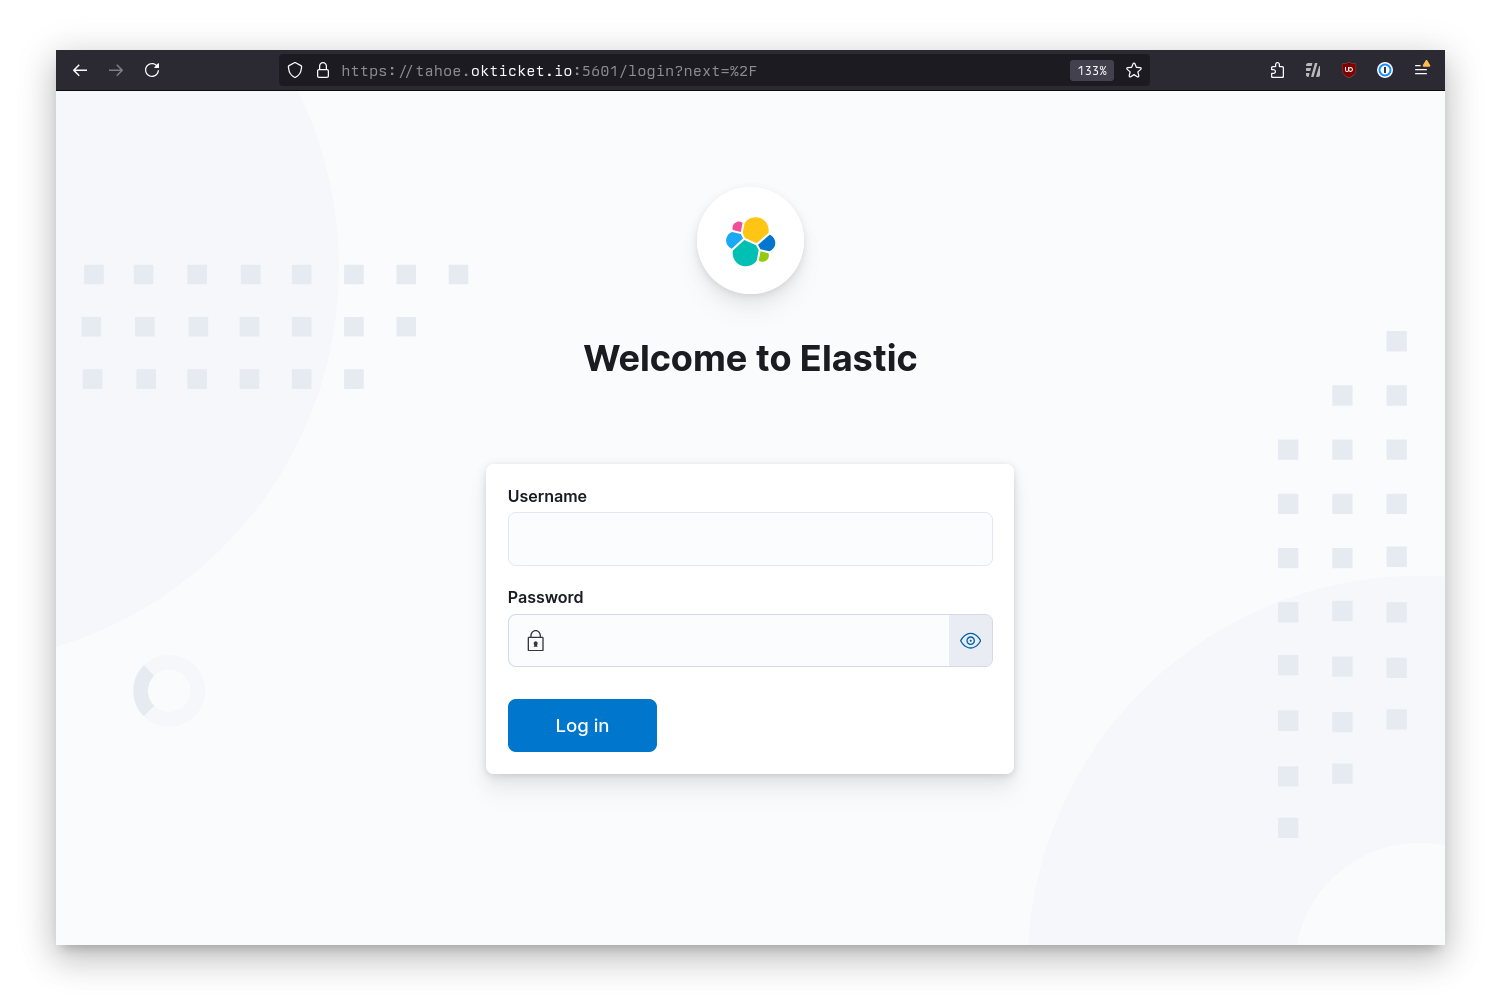
\includegraphics[width=\textwidth]{manual/kibana_login.png}
  	\caption{Pantalla de inicio de sesión de Kibana}
  \label{fig:login}
\end{figure}

\emph{NOTA: se utilizan datos y paneles de ejemplo para ilustrar el manual.}

\subsection{Usuario normal}
Una vez introducidos los datos de acceso, Kibana redirige el usuario a la
página por defecto configurada para su rol, que para el usuario final debería
ser siempre el listado de \textit{dashboards}.

\begin{figure}[H]
	\centering
  	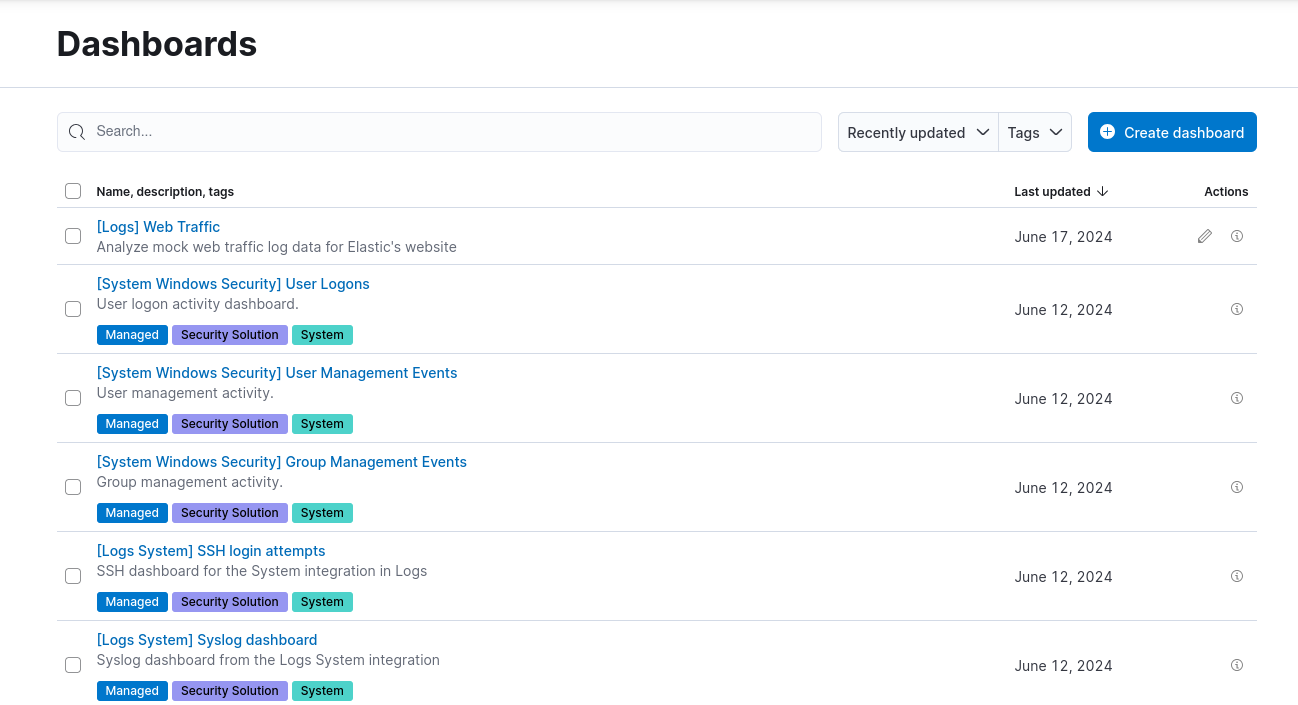
\includegraphics[width=\textwidth]{manual/dashboards.png}
  	\caption{Listado de dashboards de Kibana}
  \label{fig:dashboards}
\end{figure}

Dentro de la lista de \textit{dashboards}, el usuario puede seleccionar
cualquiera a los que tenga acceso para visualizar los datos en tiempo real.
En el caso del equipo de desarrollo, tendrán acceso a todos los paneles y
podrán modificar y crear nuevos.

\begin{figure}[H]
	\centering
  	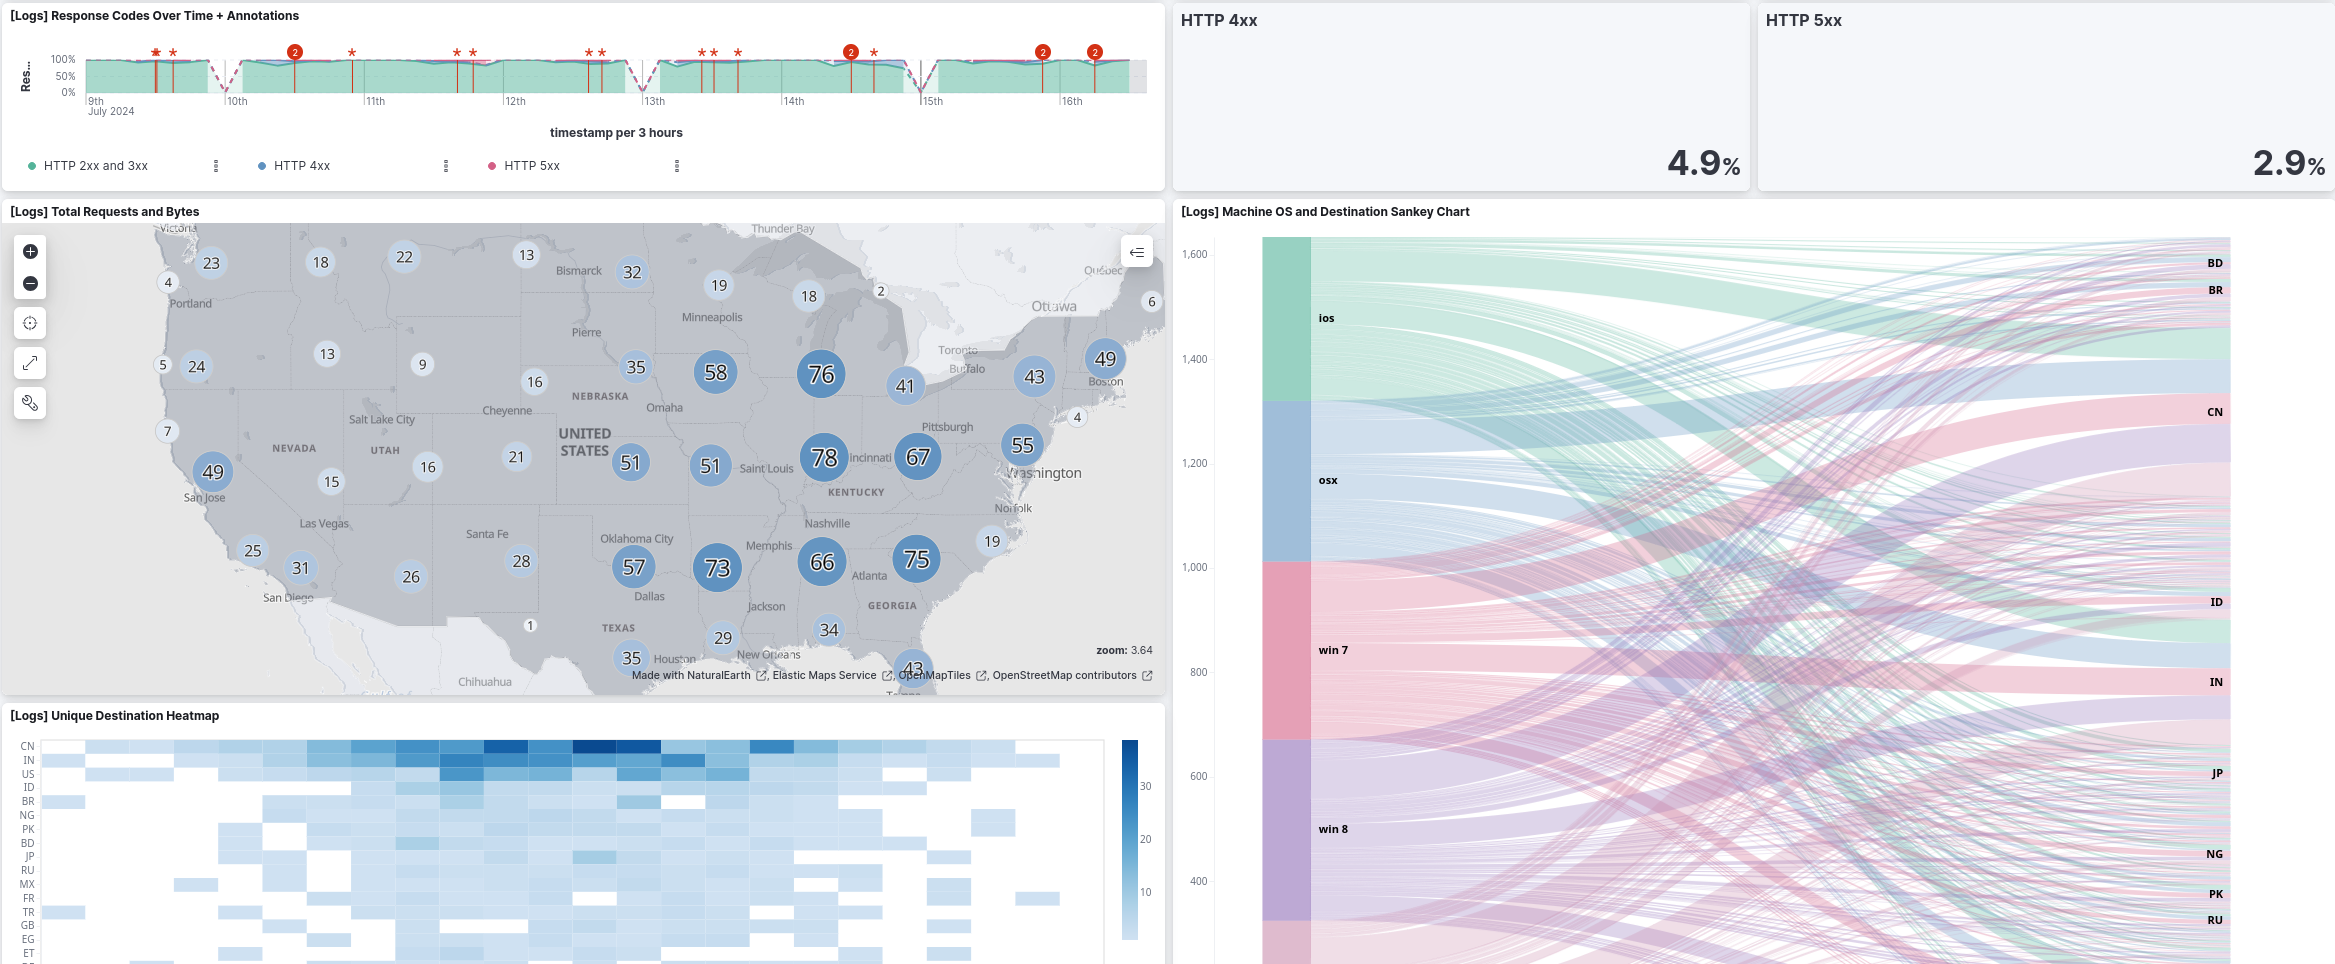
\includegraphics[width=\textwidth]{manual/dashboard.png}
  	\caption{Ejemplo de dashboard de Kibana}
  \label{fig:dashboard}
\end{figure}

En la parte superior de la pantalla, el usuario puede seleccionar el rango de
tiempo que desea visualizar, así como el intervalo de actualización de los
datos. Además, puede seleccionar el rango de tiempo de forma manual.

También existe la posibilidad de filtrar la información mostrada en el panel
según diferentes campos, bien haciendo uso de los filtros predefinidos o
haciendo consultas personalizadas en el campo de búsqueda con sintaxis KQL
\footnote{\url{https://www.elastic.co/guide/en/kibana/current/kuery-query.html}}.


\subsection{Usuario administrador}
Aquellos usuarios con permisos de administración podrán además acceder a otras
partes más avanzadas de Kibana, como la monitorización y creación de alertas o
la gestión de usuarios y roles.

\begin{figure}[H]
	\centering
  	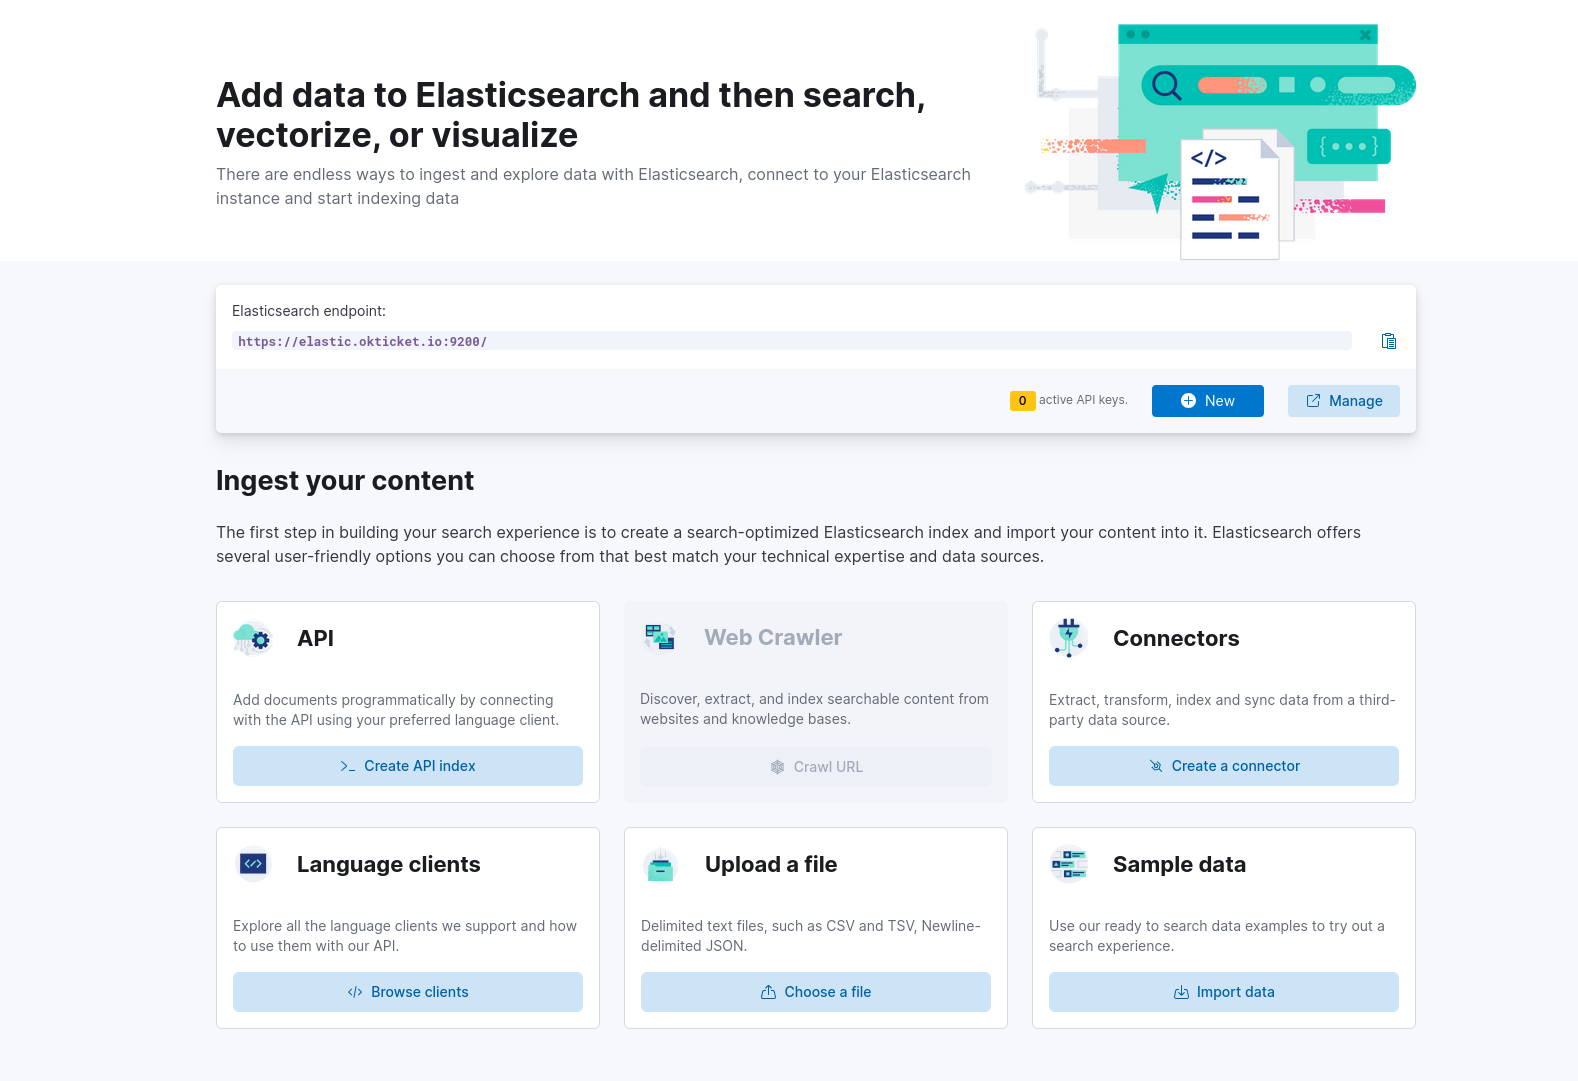
\includegraphics[width=\textwidth]{manual/kibana_config.png}
  	\caption{Opciones de fuentes de datos de Elasticsearch a través de Kibana}
  \label{fig:kibana_config}
\end{figure}

\begin{figure}[H]
	\centering
  	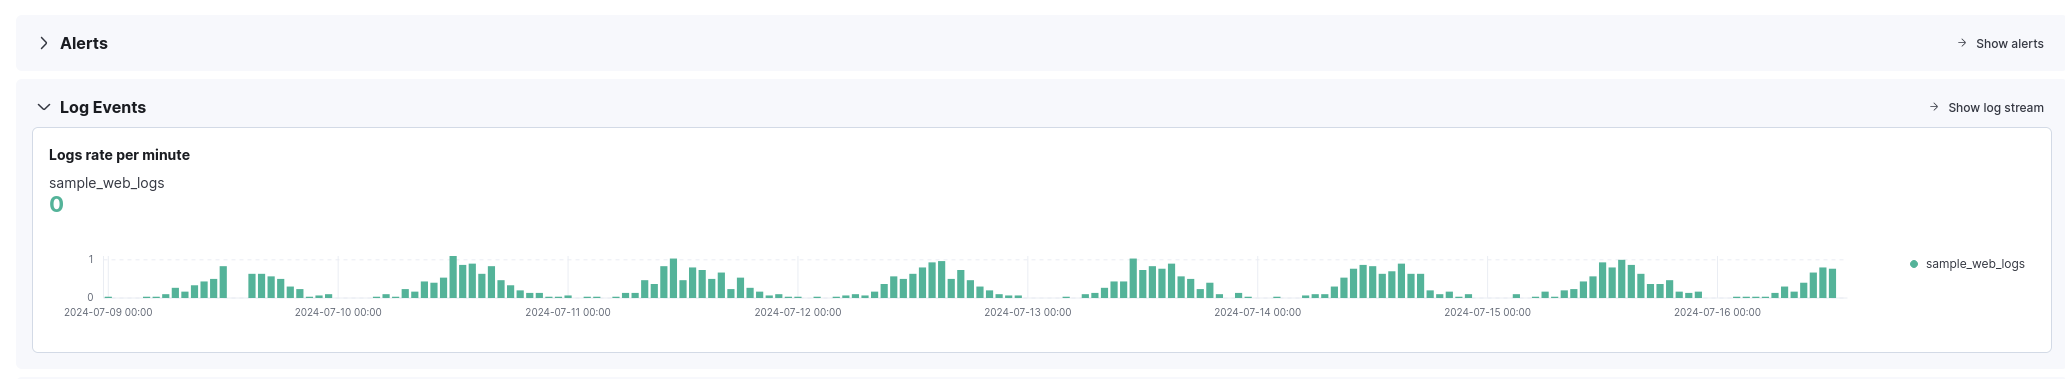
\includegraphics[width=\textwidth]{manual/kibana_alerts.png}
  	\caption{Ejemplo de alertas y métricas en Kibana}
  	\label{fig:kibana_alerts}
\end{figure}


\newpage{}
\section{Manual de despliegue}\label{sec:manual_despliegue}
El sistema se ha diseñado para llevar la menor cantidad de pasos posible en su
instalación. Debido a la colección de tecnologías utilizadas, (Terraform,
Docker y ECS), el despliegue de la infraestructura base requiere la ejecución de
tan solo dos comandos\footnote{Asumiendo que se cumplen los requisitos previos.}.

El sistema de despliegue está pensado para ser ejecutado en un sistema operativo
UNIX, como Linux o macOS. Para su ejecución en Windows, se recomienda el uso
de WSL2\footnote{\url{https://learn.microsoft.com/es-es/windows/wsl/about}}.


\subsection{Requisitos previos}
Previa al despliegue del sistema, se deben cumplir una serie de requisitos
mínimos:


\paragraph{Terraform}
El proceso de instalación de Terraform es sencillo y se puede realizar siguiendo
las instrucciones de la aplicación en su página web oficial\footnote{\url{
	https://developer.hashicorp.com/terraform/install
}} para el sistema operativo que se desee. Una vez descargado e instalado,
se puede comprobar que la instalación ha sido correcta ejecutando el comando
\texttt{terraform -v} en la terminal de comandos del sistema.

\begin{figure}[H]
	\centering
	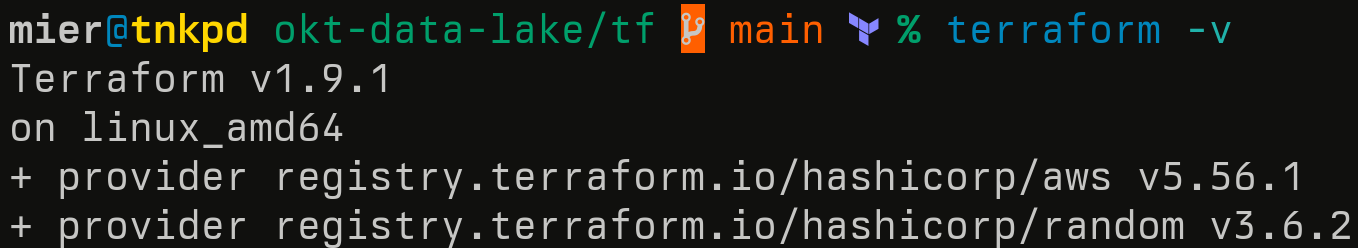
\includegraphics[width=\textwidth]{manual/terraform_v.png}
	\caption{Comprobación de la versión de Terraform}
	\label{fig:terraform_version}
\end{figure}


\newpage{}
\paragraph{Usuario de AWS}
Para poder ejecutar los comandos de Terraform con los permisos necesarios, se
debe disponer de un usuario de AWS con los permisos necesarios para la creación
de los recursos. Se recomienda la creación de un usuario específico para el
despliegue del sistema, con los roles y políticas estrictamente necesarias, para
evitar posibles problemas de seguridad.

Para permitir la interacción con la consola de AWS, se debe instalar la
herramienta de terminal de Amazon\footnote{\url{https://aws.amazon.com/es/cli/}}.

Una vez creado o seleccionado el usuario deseado, se debe inciar sesión en la
consola a través del comando \texttt{aws configure} y seguir las instrucciones
para introducir las credenciales de acceso al sistema.

\begin{figure}[H]
	\centering
	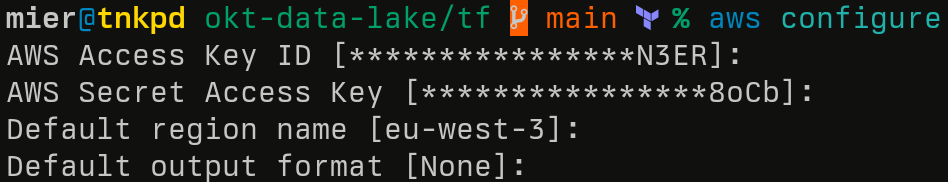
\includegraphics[width=\textwidth]{manual/aws_configure.png}
	\caption{Configuración de credenciales en AWS CLI}
	\label{fig:aws_configure}
\end{figure}

AWS pone a disposición de los usuarios una guía de inicio rápido\footnote{\url{
	https://docs.aws.amazon.com/es_es/cli/latest/userguide/cli-configure-quickstart.html
}} para la configuración de las credenciales.

\begin{figure}[H]
	\centering
	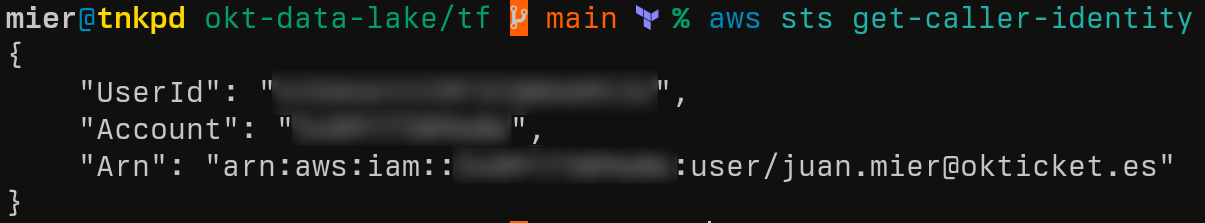
\includegraphics[width=\textwidth]{manual/aws_user.png}
	\caption{Demostración de credenciales en AWS CLI}
	\label{fig:aws_user}
\end{figure}


\newpage{}
\paragraph{Certificados}
Para que funcionen correctamente los servicios de la aplicación mediante HTTPS,
se deben disponer de certificados separados tanto para el dominio y los
recursos de AWS como para los servicios de la aplicación.

Los certificados de AWS se generan automáticamente con el script mediante el
servicio de ACM, mientras que los certificados de la aplicación se deben
generar previamente y almacenar en la carpeta \texttt{certs} del proyecto.

Para la generación de los certificados de la aplicación, se reutiliza los
scripts de preparación de los contenedores del \fullref{sec:impl_local}.
Para la generación de los certificados de la aplicación, se debe ejecutar
el script \texttt{certs.sh} que se encuentra en \fullref{anexo:certificados} o
bien se pueden reutilizar los certificados generados en el despliegue local.

Estos certificados deben ser almacenados en la carpeta \texttt{certs} junto a
los scripts de despliegue de Terraform, y deben tener visibilidad suficiente
para que Terraform pueda acceder a ellos.


\newpage{}
\subsection{Despliegue}
Una vez cumplidos los requisitos previos, se puede proceder al despliegue de
la infraestructura base. Para ello, se deben ejecutar los siguientes comandos
desde la carpeta de scripts de Terraform a través de la terminal del sistema:

\begin{lstlisting}
terraform init  # Necesario solo la primera ejecucion
terraform apply
\end{lstlisting}

\begin{figure}[H]
	\centering
	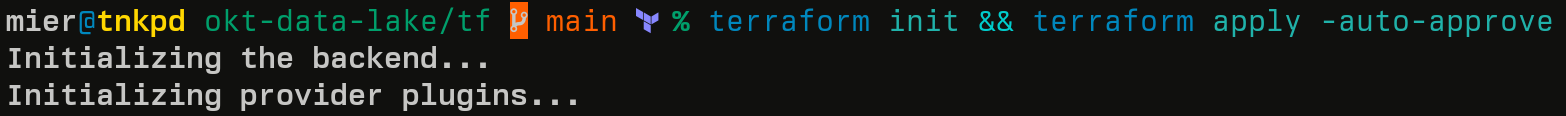
\includegraphics[width=\textwidth]{manual/terraform_apply.png}
	\caption{Despliegue de la infraestructura base}
	\label{fig:terraform_apply}
\end{figure}

El comando \texttt{terraform init} se encarga de inicializar el directorio de
trabajo de Terraform, descargando los módulos necesarios para el despliegue.
El comando \texttt{terraform apply} se encarga de desplegar la infraestructura
base en la cuenta de AWS asociada a las credenciales configuradas en la
herramienta de AWS CLI.

Una vez ejecutado el comando, se mostrará un resumen de los recursos que se
van a crear y se pedirá confirmación para proceder con el despliegue. Para
confirmar, se debe introducir \texttt{yes} y pulsar la tecla \texttt{Enter}.
Una vez confirmado, Terraform procederá a la creación de los recursos de manera
automatizada.

Una vez concluido el despliegue, se mostrará un mensaje de éxito y se devolverán
algunos datos relevantes sobre los recursos creados, como direcciones URL,
identificadores o contraseñas de acceso creadas de manera aleatoria.

\begin{figure}[H]
	\centering
	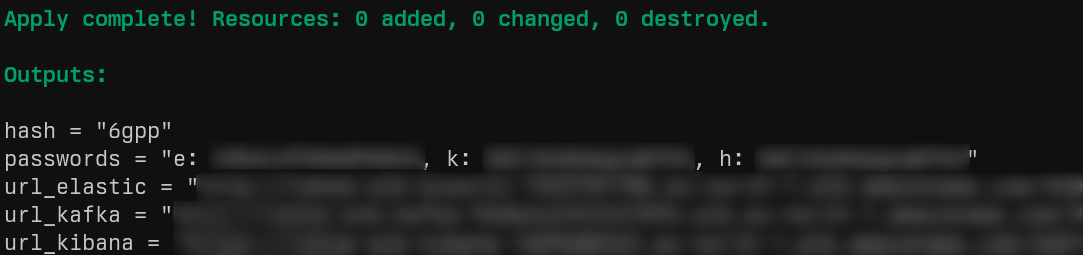
\includegraphics[width=\textwidth]{manual/terraform_output.png}
	\caption{Despliegue exitoso de la infraestructura base}
	\label{fig:terraform_output}
\end{figure}


\chapter{Resultados y trabajo futuro}
El propósito de este capítulo es presentar las conclusiones obtenidas a partir
del desarrollo del proyecto, recopilar las dificultades encontradas y proponer
líneas de trabajo futuro en vista a la amplicación y mejora del sistema.

\section{Resultados}
El resultado del proyecto es un sistema de monitorización y análisis de datos
funcional y escalable, que permite a los usuarios obtener insights valiosos a
partir de la información recopilada.

Se ha logrado implementar una arquitectura robusta y flexible, basada en
tecnologías modernas y en la nube, que facilita la ingesta, procesamiento y
visualización de datos de manera eficiente y sencilla.

El sistema es capaz de ingestar datos de diversas fuentes, como bases de datos
internas, logs de aplicaciones y servicios externos, y de presentarlos de forma
clara y útil a través de Kibana.

La infraestructura se despliega y orquesta de manera automática en la nube,
permitiendo una gestión sencilla y eficiente del sistema para los
administradores.

Pese a que no se han completado todas las historias de usuario planificadas,
se han logrado los objetivos principales del proyecto, sentando las bases para
futuras iteraciones y logrando así entregar un producto mínimo viable (MVP).

El motivo de no haber completado todas las historias de usuario planificadas
se debe al tamaño y naturaleza del proyecto, que ha resultado ser más complejo
de lo esperado en un principio. Sin embargo, se ha logrado superar los objetivos
principales y se ha entregado un producto funcional y de calidad.


\newpage{}
\section{Trabajo futuro}
El proyecto ha sentado las bases para un sistema de monitorización y análisis de
datos robusto y escalable. Sin embargo, existen áreas de mejora y ampliación que
podrían ser abordadas en futuras iteraciones.


\subsection{Historias de usuario restantes}
Lo primero de todo sería completar las historias de usuario menos críticas que
han quedado pendientes, como la ingesta de datos de APIs externas o el
\textit{web scraping}. Estas funcionalidades permitirían enriquecer los datos
disponibles y ampliar las fuentes de información.

\begin{table}[H]
	\centering
	\begin{tabular}{|p{0.7\linewidth}|c|c|}
		\hline
		\textbf{Nombre} & \textbf{Prioridad} & \textbf{Tamaño} \\
		\hline
		\hline
		Como desarrollador de Okticket, quiero que los datos contengan metadatos que faciliten su filtrado o búsqueda & P2\cellcolor{yellow!50} & XS\cellcolor{blue!25} \\
		\hline
		Como trabajador de Okticket, quiero poder ver y consultar datos de empresas cliente & P2\cellcolor{yellow!50} & S\cellcolor{green!25} \\
		\hline
		Como gestor de una empresa cliente, quiero poder ver información relevante sobre mi empresa que recoja Okticket & P2\cellcolor{yellow!50} & M\cellcolor{yellow!50} \\
		\hline
		Como desarrollador de Okticket, quiero poder ingestar datos de APIs externas a la empresa & P2\cellcolor{yellow!50} & M\cellcolor{yellow!50} \\
		\hline
		Como desarrollador de Okticket, quiero poder ingestar información de páginas web externas (\textit{scraping}) & P2\cellcolor{yellow!50} & S\cellcolor{green!25} \\
		\hline
	\end{tabular}
	\caption{Historias de usuario restantes para futuras iteraciones}
	\label{tab:remaining_tasks}
\end{table}

Como se puede observar en la tabla \ref{tab:remaining_tasks}, las historias de
usuario restantes son las menos prioritarias (siguiendo con
\fullref{sec:planif_inicial}).

\newpage{}
\subsection{Integración de lenguaje natural para búsqueda (DSL)}
Sería interesante explorar la posibilidad de integrar el sistema con
un sistema de búsqueda y filtrado de datos a través de lenguaje natural, como
\textit{Natural Language Processing} (NLP)\footnote{
	\url{https://www.elastic.co/guide/en/elasticsearch/reference/current/query-dsl-query-string-query.html}
}

Esto permitiría a los usuarios realizar consultas de manera más intuitiva y
eficiente, sin necesidad de conocer la sintaxis de Kibana Query Language (KQL).


\subsection{Aplicación de modelos de Lenguaje de Gran Escala (LLM)}
Desde la empresa, se ha propuesto la posibilidad de aplicar modelos de LLM
para la generación de texto automática, presumiblemente de manera agnóstica al
proveedor (OpenAI, Anthropic, Google\ldots).

Esto permitiría la generación de informes y análisis de manera automática a
partir de los datos recopilados, facilitando la toma de decisiones y la
comunicación de insights a los usuarios.

\subsection{Más perspectivas futuras}
Gracias a la flexibilidad del stack ELK, se podrían añadir nuevas fuentes de
datos y visualizaciones, como logs de otras partes de la aplicación (gestor web,
otros servicios internos como Hubspot o Holded, aplicación móvil\ldots) o
visualizaciones más avanzadas y personalizadas.

Lo bueno de haber diseñado la arquitectura de la manera que se ha hecho
es que se pueden añadir nuevas funcionalidades sin necesidad de modificar
la infraestructura existente, simplemente añadiendo nuevos servicios y
configuraciones.

La escalabilidad del sistema también es un punto a tener en cuenta. En caso de
necesitar más capacidad de procesamiento o almacenamiento, se podría establecer
un sistema de autoescalabilidad en base a las definiciones ya realizadas.

Por último, se podría explotar la funcionalidad del stack de generar alertas
en base a la información ingestada y procesada, para notificar a los usuarios
de eventos críticos o anomalías detectadas en los datos.


\newpage{}
\section{Conclusiones y retrospectiva}
El desarrollo de este proyecto me ha permitido, a nivel personal, adquirir
conocimientos y habilidades muy útiles en áreas que tienen una gran demanda en
el mercado laboral actual, como la ingesta y procesamiento de datos, la
orquestación de servicios en la nube y la experiencia con proveedores cloud como
AWS.

A nivel técnico, he aprendido a trabajar con tecnologías modernas y potentes,
como Kafka, Logstash, Elasticsearch y Kibana, que me han permitido implementar
una solución robusta y escalable para la monitorización y análisis de datos.

Además, he tenido la oportunidad de trabajar con metodologías ágiles y de
gestión de proyectos, como Scrum, en proyectos reales con repercusiones y
resultados tangibles.

En cuanto a la retrospectiva del proyecto, considero que el tiempo dedicado ha
merecido la pena, pero podría haber sido gestionado u organizado diferente.


%% Anexos
% \addcontentsline{toc}{chapter}{Anexos}
\appendix % Inicia los anexos
\chapter{Código de despliegue local}\label{anexo:local}
\lstinputlisting[style=yaml]{input/docker-compose.yml}
\lstinputlisting{input/.env.example}

\chapter{Script de creación de certificados}\label{anexo:certificados}
\lstinputlisting[language=bash]{input/certs.sh}
% TODO: fix estilo bash no funcional


%% Esto incluirá la bibliografía correctamente en nuestro trabajo
\newpage % En una nueva página
\addcontentsline{toc}{chapter}{Bibliografía} % Añade la referencia al índice de contenido

\bibliographystyle{ieeetr} % Define el estilo de la bibliografía
\bibliography{biblio} % Indica el archivo que contiene la colección de citas

\nocite{template}
\nocite{mier2024anomalias}

\end{document}
